\chapter{基于移动模式最优节点群组选取的路由算法}
\label{chap:基于移动模式最优节点群组选取的路由算法}

在许多节点具有一定社会属性的机会网络中,具有共同兴趣的移动用户往往访问一些与其兴趣相关的地点。研究表明,50\%的移动用户会在某一个特定的接入点(access point, AP)上花费约74\%的时间\upcite{Henderson:2004ul}。换言之,节点往往具有频繁访问某一或某一部分地点(简称为常访地点)的特点。这些常访地点可被看做``连接''这些节点的枢纽。可以通过在常访地点部署缓存设备,用以辅助消息传递,例如投掷盒(throw-box)\upcite{Ibrahim:2009we}等设备。缓存设备具有普通移动节点不具备的优势。首先,由于部署的缓存设备位置固定在常访地点,且节点往往在常访地点停留一段时间,所以节点与缓存设备之间具有比移动节点之间更加稳定的连接。其次,这些固定的缓存设备,没有如同移动节点那样便携性的限制和要求,故其存储容量往往比移动节点要大许多。由此,可以利用在常访地点部署缓存设备作为中继枢纽,从而提升机会网络中路由算法的性能表现。

本章研究多副本单播机会路由算法,基本假设如下。每条消息具有一对“源—目的”节点对(source-destination node pair),并且每条消息可在网络中具有多份拷贝。不同于以往基于社会网络分析求解社会关系的方法,或自定义社会属性的方法,本章利用节点收集的移动记录信息,从中提取出节点(群组)移动模式,并以此为依据选出最优中继节点群组。基本思想为:将持有某一条特定消息(或其拷贝)的任意一组节点看成一个整体,从记录信息中提取出移动模式,从而确定该节点群组的常访地点集合$A_1$。目的节点的常访地点$A_2$,也以相同方法获取。进而,取交集求得$A=A_1\cap A_2$,作为该节点群组与目的节点的共同常访地点集合。利用集合$A$,可以求出消息的预测投递率。路由目标即为求得能使预测投递概率最大的节点群组。此外,超出有效期(deadline)的消息不再具有价值,在求解移动模式的过程中,消息的时效性也被考虑在内。本章基于节点的移动模式,提出构造最优节点群组作为中继节点群的移动模式相关最优路由算法MPAR。就目前掌握的资料来看,这是首次利用节点群组移动模式进行社会相关的路由算法研究。

本章组织如下:第\ref{chap3:系统模型及基本定义}节引入系统模型及基本定义;第\ref{chap3:路由问题概览}节分析路由问题背后蕴含的两个关键属性,并给出最优路由问题的形式化定义;第\ref{chap3:搜索问题分析}节证明了该最优问题的计算复杂性,并提出了启发式算法用以求解近似最优解;第\ref{chap3:最优化路由算法}节给出路由算法的详细过程及描述;第\ref{chap3:仿真实验}节对仿真实验结果进行分析;第\ref{chap3:本章总结}节总结本章内容。

\section{系统模型及基本定义}
\label{chap3:系统模型及基本定义}

\begin{figure}
\centering
\subfigure[节点a向投掷盒发送消息\label{paper-MPAR/send_to_box}]
{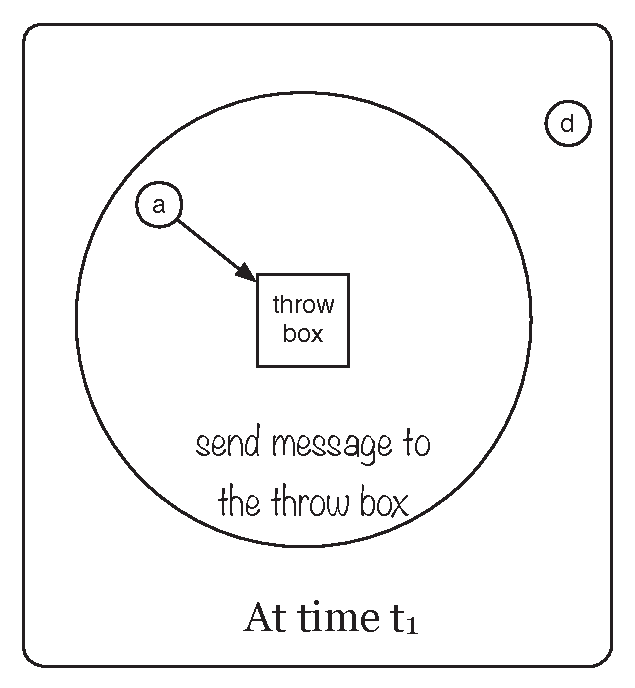
\includegraphics[width=0.4\linewidth]{paper-MPAR/send_to_box}}~~~~~~
\subfigure[节点d从投掷盒接受消息\label{paper-MPAR/receive_from_box}]
{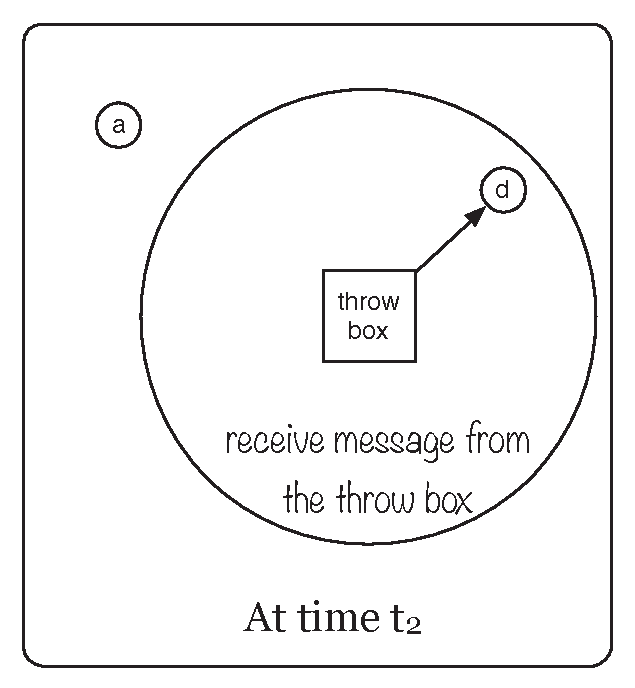
\includegraphics[width=0.4\linewidth]{paper-MPAR/receive_from_box}}
\caption{利用投掷盒完成消息从节点a到节点d的传递操作.}
\label{fig:chap3_box}
\end{figure}

\subsection{网络模型}

网络节点集合记为$\overline{N}\triangleq\{n_i|1\leq i\leq n\}$. 节点在给定的地点集合间移动,地点集合记为$\overline{A}\triangleq\{a_j|1\leq j \leq m\}$. 任意一个节点$n_i$的常访地点集合$A(n_i)\subseteq \overline{A}$. 该模型源于真实的移动网络,一个典型的实例是Dartmouth College的Wi-Fi Campus Network \upcite{Jedari:2013uo}。另一符合该模型的一类网络是VANET。在VANET中,大量的公交车,电车等在车站等固定地点间移动。我们假设节点$n_i$访问任意一个地点$a_j$的时间间隔服从指数分布。此外,在任意地点内都部署有一个投掷盒装置,用于接受,缓存及传递消息。在此模型中,投掷盒的缓存容量假设为足够大,即在投掷盒中不会因缓存满而产生消息丢弃。如\figurename~\ref{fig:chap3_box}所示,节点a在$t_1$时刻将消息托管给投掷盒,在$t_2$时刻,该消息的目的节点d进入投掷盒的传输范围内,并从投掷盒接受该消息,至此,消息的投递操作完成。

我们假设每条消息$l$都具有一个值$\tau_l$,代表消息$l$在网络的剩余生存时间。随着时间消逝,$\tau_l$的值逐渐减少,当$\tau_l=0$时,该消息将从节点缓存中删除,不再存在于网络中。消息的生存时间属性,一定程度上避免了消息在网络中停留的时间过长。此外,应用程序所产生的消息因具有时效性,往往也会对消息设定一个生存时间。例如新闻发布或者广告发布服务,消息只在一定时间内有效。当消息超出某个时间即不再具有投递价值。




\subsection{基本定义}

由于作为手持设备的节点附属于具有社交属性的人群,节点的移动模式具有一定的周期性。举例而言,Smith先生在周一到周五上班,故其常访地点可能包含家,办公室,某些公交站点及一些快餐店等。周末,Smith先生通常去健身俱乐部或咖啡馆,或者一些不同于工作时间去的地方。然而,他的行为通常以一星期为一个周期,在一定程度上重复,即其移动记录具有一定的周期性。假设周期为$T$,若将$T$划分为$h$个时间槽,则每个时间槽的长度为$\frac{T}{h}$。将这些划分好的时间槽的边界时间点,用序列$<t_0,t_1,t_2,\ldots,t_h>$表示,则任意两个区间点$t_s$与$t_e$($t_s<t_e$)形成时间区间$[t_s,t_e]$,如图\figurename~\ref{fig:chap3_time_slots}所示。针对时间区间$[t_s,t_e]$,可以从节点的移动记录中,提取出对应的移动模式。节点的移动记录见定义\ref{def:移动记录}。

\begin{figure}[!t]
\centering
  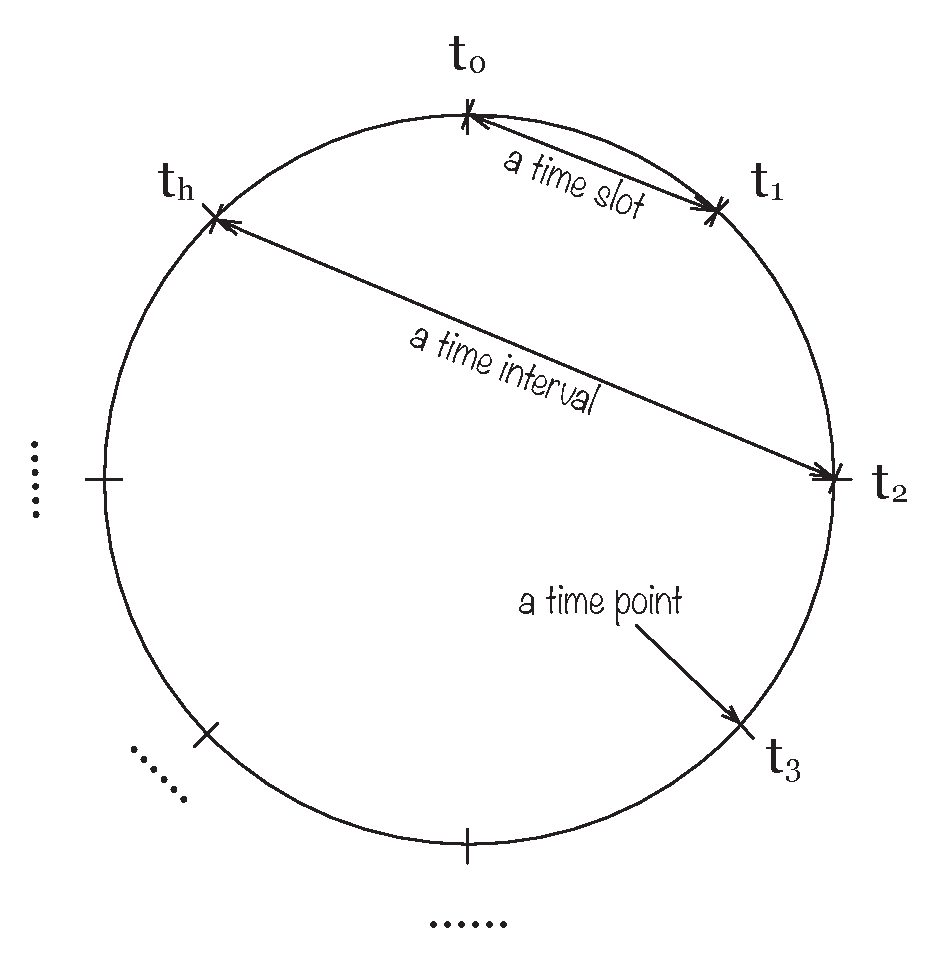
\includegraphics[width=0.55\linewidth]{paper-MPAR/time_slots}
  \caption{周期$T$划分为$h$个时间槽}
  \label{fig:chap3_time_slots}
\end{figure}

\begin{definition} 移动记录\\
节点$n_i$的移动记录定义为一个$h\times m$矩阵,记为$\mathbb{R}(i)$
\[
\mathbb{R}(i)=
\left.\left[
\overbrace{
\begin{array}{cccc}
\sfrac{1}{r_{1,1}^i} & \sfrac{1}{r_{1,2}^i} & \ldots & \sfrac{1}{r_{1,m}^i}\\
\sfrac{1}{r_{2,1}^i} & \sfrac{1}{r_{2,2}^i} & \ldots & \sfrac{1}{r_{2,m}^i} \\
\vdots & \vdots & \ddots & \vdots \\
\sfrac{1}{r_{h,1}^i} & \sfrac{1}{r_{h,2}^i} & \ldots & \sfrac{1}{r_{h,m}^i} \\
\end{array}}^{m\textnormal{个地点}}
\right]\right\}\small{h\textnormal{个时间槽}}
\]
其中第$k$行的向量$\mathbb{R}(i,k)$代表时间槽$[t_{k-1},t_{k}]$内的移动记录,且有\[\mathbb{R}(i,k)=[\sfrac{1}{r^i_{k,1}},\sfrac{1}{r^i_{k,2}},\ldots,\sfrac{1}{r^i_{k,m}}]\]其中$r^i_{k,j}$代表节点 $n_i$对地点$a_j$在时间槽$[t_{k-1},t_{k}]$内的平均访问时间间隔。
\label{def:移动记录}
\end{definition}

从上述定义可知,$\sfrac{1}{r^i_{k,j}}$代表节点$n_i$对地点$a_j$的平均访问频率。特别的,若$n_i$在时间槽$[t_{k-1},t_k]$内从未到达过$a_j$,则设定$r_{k,j}^i=\infty$,于是有$\sfrac{1}{r^i_{k,j}}=0$. 对于所有的时间槽,可以求出节点$n_i$对于地点$a_j$的平均访问时间间隔$M_{i,j}$,记为
\begin{equation}
M_{i,j}=\left.\sum_{k=1}^{k=h}r^{i}_{k,j}\middle/h\right.
\label{eq:meeting_interval}
\end{equation}

\section{路由问题概览}
\label{chap3:路由问题概览}

在讨论路由相关细节之前,先对路由问题做一个总览。在\ref{chap3:移动模式}小节中,讨论如何从一组节点中提取对应的节点群组移动模式。随后在\ref{chap3:路由相关的两个关键属性}小节中,分析路由相关的两个关键属性。最后,在\ref{chap3:路由问题形式化定义}小节中,给出最优路由问题的形式化定义。

\subsection{移动模式}
\label{chap3:移动模式}

移动模式从节点的移动记录中提取。首先定义函数$\mathbbm{E}$,用以将移动记录向量转化为对应的移动模式向量。

\begin{figure}[t]
\centering
  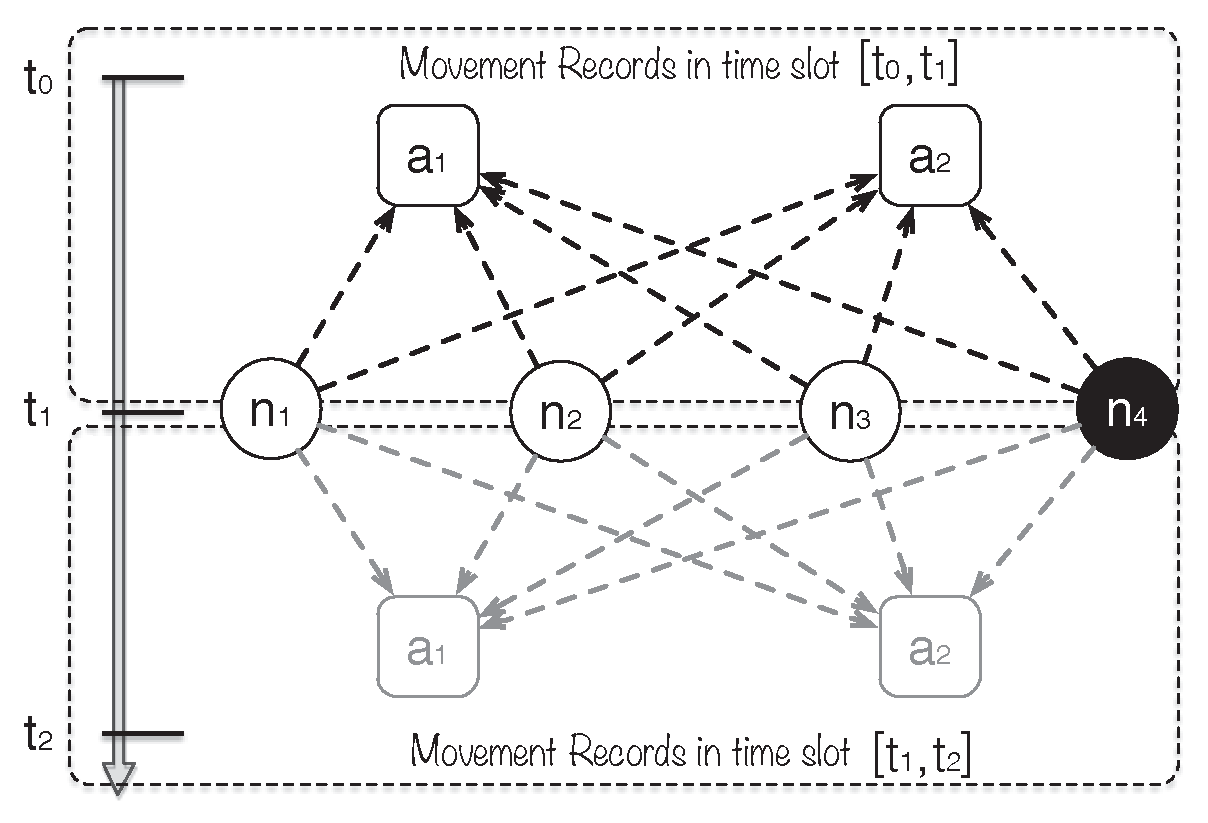
\includegraphics[width=0.7\linewidth]{paper-MPAR/example1}
  \caption{网络场景举例}
  \label{fig:chap3_example1}
\end{figure}

\begin{definition} 函数$\mathbbm{E}$
\[\mathbbm{E}([x_1,x_2,\ldots,x_m])=[\varkappa _1,\varkappa _2,\ldots,\varkappa _m]\]\textnormal{其中}
\begin{equation}
\varkappa _j=\left\{
\begin{array}{cl}
 1 &x_j\geq\frac{\updelta}{m}\sum_{i=1}^{i=m}x_i\\
 0 & otherwise
\end{array}
\right.
\label{eq:extract}
\end{equation}
\textnormal{$0<\updelta<1$ 是预设的系统参数。}
\label{def:函数E}
\end{definition}

函数$\mathbbm{E}$用于过滤节点—地点间的访问记录,不常访问的地点将被过滤掉。基于函数$\mathbbm{E}$可以直接定义移动模式,如定义\ref{def:移动模式}。

\begin{definition} 移动模式.
对于任意节点群组$N$,其在时间区间$[t_p,t_q]$ 内的移动模式,记为$\mathcal{P}(V,[t_s,t_e])$, 定义为
\begin{equation}
\mathcal{P}(N,[t_s,t_e])= \mathbbm{E}(\sum_{n_x \in N}\sum_{i=s}^{i=e}\mathbb{R}(x,t_i))
\label{eq:pattern}
\end{equation}
\label{def:移动模式}
\end{definition}

在定义\ref{def:移动模式}中,移动模式$\mathcal{P}$从某节点(群组)在某个特定时间区间$[t_s,t_e]$上的所有移动记录向量通过累加后,以函数$\mathbbm{E}$处理后得出。举例而言,假设如\figurename~\ref{fig:chap3_example1}所示的网络场景,网络中总共有四个节点$n_1,n_2,n_3,n_4$以及两个地点$a_1,a_2$。其中$n_4$是目的节点,周期$T$被划分为两个时间槽,简记为$[t_0,t_1]$与$[t_1,t_2]$。



\figurename~\ref{fig:chap3_example1}中每条边的权值如\tablename~\ref{tab:chap3_example1}所示。权值代表“节点—地点”对访问平均间隔时间。针对每个节点的记录矩阵,表示为$\mathbb{R}(1),\mathbb{R}(2),\mathbb{R}(3),\mathbb{R}(4)$。

\[
\begin{array}{cc}
\mathbb{R}(1)=\left[
\begin{array}{cc}
\sfrac{1}{2.08} & \sfrac{1}{4.65} \\
\sfrac{1}{6.02} & \sfrac{1}{2.95}
\end{array}\right]&
\mathbb{R}(2)=\left[
\begin{array}{cc}
\sfrac{1}{4.4} & \sfrac{1}{4.3} \\
\sfrac{1}{4.0} & \sfrac{1}{4.5}
\end{array}\right]    \\ \\
\mathbb{R}(3)=\left[
\begin{array}{cc}
\sfrac{1}{8.05} & \sfrac{1}{1.11} \\
\sfrac{1}{6.05} & \sfrac{1}{15.49}
\end{array}\right]
&
\mathbb{R}(4)=\left[
\begin{array}{cc}
\sfrac{1}{2.6} & \sfrac{1}{3.3} \\
\sfrac{1}{3.5} & \sfrac{1}{3.5}
\end{array}\right]
\end{array}
\]

\begin{table}[hbt]
\centering
  \caption{网络场景\figurename~\ref{fig:chap3_example1}边权值}
  \begin{tabular}{|c|c|cc|}
  \hline
    & & $a_1$ & $a_2$  \\
    \hline
    
    %%t1
    \multicolumn{1}{|c|}{\multirow{4}{*}{$[t_0,t_1]$}} & $n_1$ &2.08 & 4.65 \\
    & $n_2$ & 4.4 & 4.3 \\
    & $n_3$ & 8.05 & 1.11 \\
    & $n_4$ & 2.6 & 3.3 \\
    \hline

    %%t2
    \multicolumn{1}{|c|}{\multirow{4}{*}{$[t_1,t_2]$}} & $n_1$ &6.02 & 2.95 \\
    & $n_2$ & 4.0 & 4.5 \\
    & $n_3$ & 6.05 & 15.49 \\
    & $n_4$ & 3.5 & 3.5 \\
    \hline
  \end{tabular}
  \label{tab:chap3_example1}
\end{table}
节点集合$\{n_1,n_2,n_3\}$的移动模式,可以利用公式\ref{eq:pattern}从对应的移动记录中提取出来。对应的移动记录累加计算如下:
\begin{multline*}
\sum_{i=1}^{i=3}\sum_{j=1}^{j=2}\mathbb{R}(i,j) = \left[\frac{1}{2.08}+\frac{1}{4.4}+\frac{1}{8.05}+\frac{1}{6.02}+\frac{1}{4.0}+\frac{1}{6.05},\right.\\
\left.\frac{1}{4.65}+\frac{1}{4.3}+\frac{1}{1.11}+\frac{1}{2.95}+\frac{1}{4.5}+\frac{1}{15.49}\right]= [1.414,1.974]
\end{multline*}
针对公式\ref{eq:extract},设定参数$\delta=0.95$,从定义\ref{def:函数E}得出
\[
\frac{\updelta}{m}\sum_{i=1}^{i=m}v_i=\frac{0.95}{2}\times(1.414+1.974)\approx 1.609
\] 
所得值1.609大于向量第一个元素值1.414,且小于向量第二个元素值1.974,故对应移动模式提取如下
\[
\mathcal{P}(\{n_1,n_2,n_3\},[t_0,t_2])=[0,1] 
\]

移动模式$\mathcal{P}$指明了节点群组$\{n_1,n_2,n_3\}$在时间区间$[t_0,t_2]$内的的常访区域集合,即$A(\{n_1,n_2,n_3\},[t_0,t_2])=\{a_2\}$。对于集合$\overline{N}\\\{n_d\}$,共有$2^{n-1}-1$个非空子集,每一个子集可被看做用于向目的节点$n_d$合作投递消息的一个整体。在本例中,基于移动记录,提取出非空节点集$\{n_1,n_2,n_3\}$以及目的节点$n_4$的移动模式,结果如下\\
\begin{center}
\begin{tabular}{ll}
 & \\
$\mathcal{P}(\{n_1\},[t_0,t_2])=[1,0]$ & $\mathcal{P}(\{n_1,n_2\},[t_0,t_2])=[1,0]$ \\
$\mathcal{P}(\{n_2\},[t_0,t_2])=[1,1]$ & $\mathcal{P}(\{n_1,n_3\},[t_0,t_2])=[0,1]$ \\
$\mathcal{P}(\{n_3\},[t_0,t_2])=[0,1]$ & $\mathcal{P}(\{n_2,n_3\},[t_0,t_2])=[0,1]$ \\
$\mathcal{P}(\{n_4\},[t_0,t_2])=[1,1]$ & $\mathcal{P}(\{n_1,n_2,n_3\},[t_0,t_2])=[0,1]$ \\
 &
\end{tabular}
\end{center}
对应的常访地点集合,如下
\begin{center}
\begin{tabular}{ll}
 & \\
$A(\{n_1\},[t_0,t_2])=\{a_1\}$ & $A(\{n_1,n_2\},[t_0,t_2])=\{a_1\}$ \\
$A(\{n_2\},[t_0,t_2])=\{a_1,a_2\}$ & $A(\{n_1,n_3\},[t_0,t_2])=\{a_2\}$ \\
$A(\{n_3\},[t_0,t_2])=\{a_2\}$ & $A(\{n_2,n_3\},[t_0,t_2])=\{a_2\}$ \\
$A(\{n_4\},[t_0,t_2])=\{a_2\}$ & $A(\{n_1,n_2,n_3\},[t_0,t_2])=\{a_1,a_2\}$ \\
 &
\end{tabular}
\end{center}
\subsection{路由相关的两个关键属性}
\label{chap3:路由相关的两个关键属性}

\subsubsection{投递概率}

设节点集合$N$在时间区间$[t_0,t_0+t_l]$内的移动模式为$P(N,[t_0,t_0+t_l])$,目的节点$n_d$的移动模式为$\mathcal{P}(n_d,[t_0,t_0+\tau_l])$,共同常访地点集合记为$A$,则有$A=A(N,[t_0,t_0+\tau_l])\cap A(n_d,[t_0,t_0+\tau_l])$。记任意地点$a_j$及任意节点$n_i\in N$满足节点$n_i$和$n_d$
都在某一时间访问$a_j$。设随机变量$T_{i,j}$及$T_{d,j}$分别代表$n_i$和$n_d$到达$a_j$的时间,若要使消息能够成功传递,则须满足$T_{i,j}<T_{d,j}<\tau_l$,换言之,$n_i$须先于$n_d$到达$a_j$托管消息,且$n_d$需在消息到期之前到达$a_j$取出消息。为了便于讨论,设起始时间点$t_0=0$。此外,如\ref{chap3:系统模型及基本定义}节所述,任意节点访问任意地点的时间间隔服从指数分布。从公式\ref{eq:meeting_interval}可以计算出节点$n_i$访问地点$a_j$的指数分布参数$\lambda_{i,j}$,即

\[
\lambda_{i,j} = \sfrac{1}{M_{i,j}}
\]

对于$A$为空集的情形,默认其预测投递概率为0,到达其它地点的期望时延为$\infty$。对于$A$非空的情形,可依公式(\ref{eq:probability})预测节点$n_i$对$n_d$的投递率。进一步的,节点集$N$对$n_d$的投递率可依公式(\ref{eq:probability2})预测。
\begin{multline}
P_{i,d}=1-\prod_{a_j\in A}\left(1-P(T_{i,j}<T_{d,j}<\tau_l) \right) \\
=1-\prod_{a_j\in A}\left(1-\int _{0}^{\tau _l}\!\!\!\!\int _{t_{i,j}}^{\tau _l}f_{T_{i,j},T_{d,j}}\left(t_{i,j},t_{d,j}\right)dt_{d,j}dt_{i,j}\right)\\
=1-\prod_{a_j\in A}\left(1-\int _{0}^{\tau _l}\!\!\!\!\int _{t_{i,j}}^{\tau _l}f_{T_{i,j}}(t_{i,j})f_{T_{d,j}}(t_{d,j}) dt_{d,j}dt_{i,j}\right) \\
=1-\prod_{a_j\in A}\left(1-\int _{0}^{\tau _l}\!\!\!\!\int _{t_{i,j}}^{\tau _l}\lambda _{d,j} \lambda _{i,j} e^{-\left(\lambda _{d,j}t_{d,j}+\lambda _{i,j}t_{i,j}\right)}dt_{d,j}dt_{i,j}\right)\\
=1-\prod_{a_j\in A}\left(1-\frac{\lambda _{i,j} \left(1-e^{-\tau _l \left(\lambda _{d,j}+\lambda _{i,j}\right)}\right)}{\lambda _{d,j}+\lambda _{i,j}}
-\left(e^{\tau _l \lambda _{i,j}}-1\right) e^{-\tau _l \left(\lambda _{d,j}+\lambda _{i,j}\right)}\right)
\label{eq:probability}
\end{multline}
\begin{multline}
P_{N,d}=1-\prod_{n_i\in N}(1-P_{i,d}) \\
=1-\prod_{n_i\in N}\prod_{a_j\in A}\left(1-\frac{\lambda _{i,j} \left(1-e^{-\tau _l \left(\lambda _{d,j}+\lambda _{i,j}\right)}\right)}{\lambda _{d,j}+\lambda _{i,j}}
-\left(e^{\tau _l \lambda _{i,j}}-1\right) e^{-\tau _l \left(\lambda _{d,j}+\lambda _{i,j}\right)}\right)
\label{eq:probability2}
\end{multline}
特别而言,当消息生存时间设为无穷时,即$\tau_l=\infty$,有
\begin{multline}
P_{i,d} = 1-
\prod_{a_j\in A}\left(1-\int _0^{\infty }\!\!\!\!\int _{t_{i,j}}^{\infty }\lambda _{d,j} \lambda _{i,j} e^{-\left(\lambda _{d,j} t_{d,j}+\lambda _{i,j} t_{i,j}\right)}dt_{d,j}dt_{i,j} \right)\\
=1-\prod_{a_j\in A}\left(1-\frac{\lambda _{i,j}}{\lambda _{d,j}+\lambda _{i,j}}\right)
\label{eq:probability_infty}
\end{multline}
对于$P_{N,d}$,有
\begin{equation}
P_{N,d} = 1-\prod_{n_i\in N}\prod_{a_j\in A}\left(1-\frac{\lambda _{i,j}}{\lambda _{d,j}+\lambda _{i,j}}\right) 
=1-\prod_{n_i\in N}\prod_{a_j\in A}\frac{\lambda _{d,j}}{\lambda _{d,j}+\lambda _{i,j}}
\label{eq:probability2_infty}
\end{equation}

对于\figurename~\ref{fig:chap3_example1}中的例子,为简便起见,讨论$\tau_l=\infty$的情况(形式化定义时,会给出一般情况下的定义)。对于节点集合$\{n_1,n_2,n_3\}$而言,常访地点集合$A(N,[t_0,t_3])=\{a_2\}$;对于目的节点$n_d$而言,其常访地点集合$A(n_4,[t_0,t_3])=\{a_1,a_2\}$;由此可得出共同常访地点$A=\{a_2\}$。每一个“节点—地点”对的平均访问时间间隔,可从公式(\ref{eq:meeting_interval})获得,即

\[
\begin{array}{llll}
M_{1,1}=4.05 & M_{2,1}=4.2 & M_{3,1}=7.05 & M_{4,1}=3.05 \\
M_{1,2}=3.8 & M_{2,2}=4.4 & M_{3,2}=8.3 & M_{4,2}=3.4
\end{array}
\]

由以上计算结果,可预测节点集合$N$的投递概率,如下

\begin{multline*}
P_{\{n_1,n_2,n_3\},4}=
1-\left(\frac{\lambda_{4,2}}{\lambda_{1,2}+\lambda_{4,2}}\middle)\middle(\frac{\lambda_{4,2}}{\lambda_{2,2}+\lambda_{4,2}}\middle)\middle(\frac{\lambda_{4,2}}{\lambda_{3,2}+\lambda_{4,2}}\right) \\
= 1-\left(\frac{M_{1,2}}{M_{1,2}+M_{4,2}}\middle)\middle(\frac{M_{2,2}}{M_{2,2}+M_{4,2}}\middle)\middle(\frac{M_{3,2}}{M_{3,2}+M_{4,2}}\right) 
= 0.789
\end{multline*}

\subsubsection{期望时延}

除了投递概率之外,另一个关键的属性即节点移动到其他地点的期望时延。设节点$n_i$的常访地点集合为$A_i$,用随机变量$D_i$代表$n_i$移动到下一个地点$a_j\in A_i$的期望时延。形式上,有$D_i=\min\{T_{i,1},T_{i,2},\ldots,T_{i,|A_i|}\}$,由此可求得$D_i$的概率密度函数为
\[f_{D_i}(t)=\sum_{a_k\in A_i}\lambda_{i,k}\prod_{a_h\in A_i}e^{-\lambda_{i,h}t}\]
于是有
\begin{multline}
E[D_i]=\int_{-\infty}^{\infty}tf_{D_i}(t)dt 
=\sum_{a_k\in A_i}\int_{0}^{\infty}t\lambda_{i,k}\prod_{a_h\in A_i}e^{-\lambda_{i,h}t}dt \\
=\sum_{a_k\in A_i}\frac{\lambda_{i,k}}{\left(\sum_{a_k\in A_i}\lambda_{i,h}\right)^2}
=\frac{1}{\sum_{a_k\in A_i}\lambda_{i,k}}
\label{eq:delay}
\end{multline}
对于\figurename~\ref{fig:chap3_example1}所示例子,可以分别对节点$n_1$, $n_2$及$n_3$根据公式(\ref{eq:delay})计算期望时延$E[D_i]$。
\[
\begin{array}{l}
E[D_1]=\sfrac{1}{\lambda_{1,1}}=M_{1,1}=4.05\\
E[D_2]=\frac{1}{\lambda_{2,1}+\lambda_{2,2}}=\frac{M_{2,1}M_{2,2}}{M_{2,1}+M_{2,2}}=2.15\\
E[D_3]=\sfrac{1}{\lambda_{3,2}}=M_{3,2}=8.3 
\end{array}
\]
对于任意一对节点$n_i$和$n_j$,若$E[D_i]<E[D_j]$,则从期望意义上讲,$n_i$到达下一个新地点的时间要早于$n_j$,这意味着$n_i$能够更早的将消息托管到新的投掷盒。在机会网络中多使用多拷贝策略进行路由,快速的向网络中传播足够数目的消息副本,对提升路由性能至关重要。期望时延$E[D]$是一个很好的衡量指标,应尽可能的利用$E[D]$较小的节点分发消息。在本章提出的基于局部搜索的路由算法Local-MPAR中,$E[D]$被用于衡量节点作为网络中唯一的活跃节点是否合适。在基于禁忌搜索的路由算法Tabu-MPAR中,$E[D]$被用作向网络中非对称喷洒消息副本的衡量指标。在\tablename~\ref{tab:chap3_example1}所示例子中,节点$n_2$最适合作为活跃节点,因为其期望时延$E[D]$最低,因此在期望意义上,$n_2$可以较早的将消息拷贝托管给其它地点的投掷盒。

\subsection{路由问题形式化定义}
\label{chap3:路由问题形式化定义}

机会网络中的路由问题,其优化目标可有多种。衡量路由算法性能的最主要的两个指标,即是消息投递率和平均端到端时延。尽管端到端时延在路由优化中被看做一项非常重要的指标,但路由的性能表现仍需要以可被接受的投递概率为基础。换言之,较高的投递概率是保证网络正常工作的基础。本章意图最大化消息的投递概率,进而提高路由性能表现。即寻找子集$N\subseteq\overline{N}$,从而使得$P_{N,d}\geq P_{N',d}$对于$\forall N'\subseteq\overline{N}$成立,其中$n_d$是消息的目的节点。

在\figurename~\ref{fig:chap3_example1}所示例子中,可依\ref{chap3:路由相关的两个关键属性}小节中公式(\ref{eq:probability2}),预测集合$\{n_1,n_2,n_3\}$所有非空子集的投递率,如下
\[
\begin{array}{ll}
P_{\{n_1\},4}=0.430 & P_{\{n_1,n_2\},4}=0.670  \\
P_{\{n_2\},4}=0.673 & P_{\{n_2,n_3\},4}=0.600  \\
P_{\{n_3\},4}=0.291 & P_{\{n_1,n_3\},4}=0.626  \\
P_{\{n_1,n_2,n_3\}}=0.789\\
\end{array}
\]

在本例中,最优集合即$\{n_1,n_2,n_3\}$。注意计算结果为估计投递率,并不直接与持有该消息的节点数目成正比。投递率$P_{N,d}$基于节点集合$N$,$N$在整个路由过程中被看做一个整体。对于某个$N'\subset N$而言,概率$P_{N,d}<P_{N',d}$是可能发生的。事实上,如\figurename~\ref{fig:chap3_example1}所示,对于集合$\{n_2,n_3\}$而言,其预测投递率低于集合$\{n_2\}$的预测投递率。如果忽略缓存限制和能耗资源,向整个网络中广播每条消息会获得最好的性能表现,因为在这种情况下增加中继节点的数目,可以提高消息的投递率(或者说至少不可能降低)。然而这种理想的情况在机会网络中往往并不存在。真实情况下,往往倾向于选择能够符合一定移动模式的最小节点群组,对消息进行投递。从例中可以看出,如果把持有该消息的所有节点视为一个整体,则其预测投递率被两项指标所影响:(1)节点集对应的移动模式,(2)节点集的大小。在正式定义路由问题之前,首先给出最优节点集合$N_{opt}$的定义。

\begin{definition} The optimal set $N_{opt}$\\
最优集合$N_{opt}$包含网络中的一组节点, 且有
\begin{displaymath}
N_{opt}= \min\{\mathrel{\mathop{\arg\max}\limits_{N\subseteq \overline{N}}}P_{N,d}\}
\end{displaymath}
\end{definition}

最优集合是能够取得最高预测投递率的最小集合,集合中的节点以合作的方式将消息传递给目的节点。基于此,可定义最优路由问题。

\begin{definition}$N_{opt}$搜索问题.\\
令$f(\mathbf{x})$代表目标函数, $g(\mathbf{x})$代表限制函数, 其中决策变量表示为$\mathbf{x}=\{x_1,x_2,\ldots,x_n\}$,有 
\begin{tabular}{l}
\parbox{\linewidth}{
\begin{multline*}
f(\mathbf{x})=\sum_{i=1}^{i=n}x_i\log\left(\prod_{a_j\in A}\left(1-\frac{\lambda _{i,j} \left(1-e^{-\tau _l \left(\lambda _{d,j}+\lambda _{i,j}\right)}\right)}{\lambda _{d,j}+\lambda _{i,j}}\right.-\left.\left(e^{\tau _l \lambda _{i,j}}-1\right) e^{-\tau _l \left(\lambda _{d,j}+\lambda _{i,j}\right)}\right)\right)
\end{multline*}
}
\end{tabular}
\[
g(\mathbf{x})=\left|\sum_{i=1}^{i=n}x_i\right|
\]
于是问题可以被形式化为如下
\[
\begin{array}{c}
\min f(\mathbf{x}) \\
s.t.\forall\mathbf{x'},~g(\mathbf{x'})-g(\mathbf{x})\geq 0, \\
\forall i,x_i\in \{0,1\}
\end{array} 
\]
当求出最优节点集合$\mathbf{x}_{opt}$时,有
\[
N_{opt}=\{n_i|x_i>0,1\leq i\leq n\}
\]
\label{def:N_opt}
\end{definition}

在上述定义中,存在一个$\bm{x}$与$N$之间的一对一映射。事实上,有$f(\bm{x})=\log(1-P_{N,d})$,其中$f(\bm{x})$与$P_{N,d}$成负相关。由此,$N_{opt}$搜索问题被形式化为最优化问题。

\section{$N_{opt}$搜索问题分析}
\label{chap3:搜索问题分析}

本节讨论$N_{opt}$问题的计算复杂性,并提出了一种启发式方法,以近似计算最优解。首先证明对于在线算法(online algorithm),对于算法输入序列中新加入的元素,能够很大程度改变目标函数的值。对于离线算法(offline algorithm),给出了$\mathcal{NP}$-hard性质证明。最后,本章提出基于禁忌搜索的启发式算法。

\subsection{计算复杂性证明}
在线算法可以分片处理输入序列。换言之,算法的输入是以一个序列方式随时间交付由算法本身处理的,而不同于离线算法,需要一次接受整个算法输入。对于$N_{opt}$,其在线算法的输入是网络中节点的移动记录,简单表示为$\mathbb{R}_{1},\mathbb{R}_{2},\ldots,\mathbb{R}_{q}$ (其中序列中的每个元素都是一个向量,例如对于在时间槽$t_i$的节点$n_x$可以有$\mathbb{R}_j=\mathbb{R}(x,t_i)$)。假设当前只有序列的前$1--k$个元素被输入算法。剩下的问题即探究当下一个新元素$\mathbb{R}_{k+1}$被加入网络时,会在多大程度上影响目标函数的值, 见定理~\ref{thm:online}

\begin{theorem}
对于$\forall k\in[1,z)$, 即使序列的前$1$---$k$部分已知,新加入的元素$\mathbb{R}_{k+1}$仍可能将移动模式改变为至少有一个元素不为0的任意向量。
\label{thm:online}
\end{theorem}
\begin{proof}
将任意向量$R_i$表示为如下
\[
R_i=[r^i_1,r^i_2,\ldots,r^i_m]~~~\forall j\in[1,m], r^i_j\geq 0
\]
向量$\sum_{i=1}^{i=k}\mathbb{R}_{i}$ 表示为
\[
\sum_{i=1}^{i=k}\mathbb{R}_{i}=[S^{k}_1,S^{k}_2,\ldots,S^{k}_m]
\]
于是对于$\forall i\in [1,m]$及 $k\in [1,z)$ 有
\[
S^{k+1}_i=S^{k}_i+r^{k+1}_i
\]
相应地,用 $\mathcal{P'}=\mathbbm{E}(\sum_{i=1}^{i=k+1}\mathbb{R}_{i})$ 和 $\mathcal{P}=\mathbbm{E}(\sum_{i=1}^{i=k+1}\mathbb{R}_{i})$ 分别表示在加入新元素$\mathbb{R}_{k+1}$之前和之后的移动模式向量。 现证明对于任意的$\mathcal{P}$, 都存在一个可能的新元素$\mathbb{R}_{k+1}$,能使向量$\mathcal{P'}$ 变为 $\mathcal{P}$.
当已知$\mathcal{P}=[\varkappa _1,\varkappa _2,\ldots,\varkappa _m]$时, 显然$\mathbb{R}_{k+1}$存在,当且仅当如下线性不等式组成立
\begin{displaymath}
\forall i\in[1,m]~~~~
\left\{
\begin{array}{ll}
S^{k+1}_i\geq\delta\sum_{j=1}^{j=m}\left(\sfrac{S^{k+1}_j}{m}\right)& \varkappa_i=1 \\
S^{k+1}_i<\delta\sum_{j=1}^{j=m}\left(\sfrac{S^{k+1}_j}{m}\right) & \varkappa_i=0
\end{array}
\right.
\end{displaymath}
即
\[
\left\{
\begin{array}{ll}
\sum_{j=1}^{j=m}r_j^{k+1}-\frac{m}{\delta}r_i^{k+1}\leq \frac{m}{\delta}S_i^{k}-\sum_{j=1}^{j=m}S_j^{k} & \varkappa_i=1 \\
\sum_{j=1}^{j=m}r_j^{k+1}-\frac{m}{\delta}r_i^{k+1}> \frac{m}{\delta}S_i^{k}-\sum_{j=1}^{j=m}S_j^{k} & \varkappa_i=0 \\
\end{array}\right.
\]

对于 $\forall i$, 将 $\frac{m}{\delta}S_i^{k}-\sum_{j=1}^{j=m}S_j^{k}$ 表示为 $w_i$, 并将$\varkappa_i=1$ 和 $\varkappa_i=0$ 时的$w_i$分别表示为 $w_{i|\varkappa_i=1}$ 和$w_{i|\varkappa_i=0}$。 同理,用 $r_i^{k+1}$ 表示 $\varkappa_i=1$ 和 $\varkappa_i=0$ 时的对应状态,有
\begin{equation}
\sum_{j=1}^{j=m}r_j^{k+1}-\frac{m}{\delta}r_{i|\varkappa_i=0}^{k+1}> w_{i|\varkappa_i=0}  
\label{eq:varkappa_0}
\end{equation}
且有
\begin{equation}
\sum_{j=1}^{j=m}r_j^{k+1}-\frac{m}{\delta}r_{i|\varkappa_i=1}^{k+1}\leq w_{i|\varkappa_i=1}
\label{eq:varkappa_1}
\end{equation}
令 $r^{k+1}_{i|\varkappa_i=0}=0$ 及 $\sum_{j=1}^{j=m}r_j^{k+1}=\max\{w_i\}+\epsilon~(\epsilon>0)$, 则等式(\ref{eq:varkappa_0})对于 $\forall \varkappa_i=0$都成立。

接下来证明可以选择足够大的$\epsilon$值,使得等式\ref{eq:varkappa_1}成立,即只需让 $\sum_{j=1}^{j=m}r_j^{k+1}-\frac{m}{\delta}r_{i|\varkappa_i=1}^{k+1}\leq \min\{w_i\}$ 对于 $\forall \varkappa_i=1$都成立,即
\[
\max\{w_i\}+\epsilon-\frac{m}{\delta}r_{i|\varkappa_i=1}^{k+1}\leq \min\{w_i\}
\]
从上述讨论, 只需让下述不等式同时成立.
\begin{equation}
r_{i|\varkappa_i=1}^{k+1}\geq\frac{\delta}{m}(\max\{w_i\}-\min\{w_i\}+1)~(0<\delta<1)
\label{eq:q1}
\end{equation}
\begin{equation}
\sum_{j=1}^{j=m}r_{j|\varkappa_j=1}^{k+1}=\max\{w_i\}+\epsilon
\label{eq:q2}
\end{equation}
假设$\mathcal{P}$中 $\varkappa_i=1$ 的数量是 $z$, 由于 $0<z\leq m$, 有
\[
z\cdot\frac{\delta}{m}(\max\{w_i\}-\min\{w_i\}+\epsilon) \leq  
\delta(\max\{w_i\}-\min\{w_i\}+\epsilon) 
\]
为使等式(\ref{eq:q1})和(\ref{eq:q2})同时成立, 只须有
\[
\delta(\max\{w_i\}-\min\{w_i\}+\epsilon) < \max\{w_i\}+\epsilon = \sum_{j=1}^{j=m}r_{j|\varkappa_j=1}^{k+1}
\]
即
\[
\epsilon>\frac{\delta}{\delta-1}\min\{w_i\}-\max\{w_i\}
\]
证毕
\end{proof}

定理~\ref{thm:npc}~给出$N_{opt}$计算复杂性的证明。

\begin{theorem}
$N_{opt}$问题属于$\mathcal{NP}$-hard类. 
\label{thm:npc}
\end{theorem}
\begin{proof}
%We reduce the $N_{opt}$ Search Problem as a Subset Sum Problem (SSP). Assume that we know a solution for a certain SSP instance of which all the elements are denoted by $R={r_1,r_2,\ldots,r_n}$ and the target value is $v$. For clarity, we transform $R$ as follows:
将子集和问题(Subset Sum Problem, SSP)归约为$N_{opt}$问题。假设已知SSP问题的一个解实例,用 $R={r_1,r_2,\ldots,r_n}$,目标值用$v$表示。为清楚起见,将$R$变为如下形式
\begin{displaymath}
R=\{\log 2^{r_1},\log 2^{r_2},\ldots,\log 2^{r_n}\}
=\{\log g_1,\log g_2,\ldots,\log g_n\}
\end{displaymath}
其中有 $g_i=2^{r_i}~~(i\in[1,n])$.
将其所有非空子集表示为 $R_1,R_2\ldots, R_{2^{|N|-1}}$。接下来,构造对应的 $N_{opt}$ 实例。 目标值为$P=v$, 节点集合为$N={n_1,n_2,\ldots,n_n}$, 对应上述提到的集合$R$. 对于每一个$N$的非空子集$N_i$, 都存在一个$R$的子集$R_i$与其一一对应 (所有的角标都是一一对应的), 将任意子集$N_j$表示为如下
\[
N_j=\{n_{j_1},n_{j_2},\ldots,n_{j_k}\}
\]
对于$\forall j$, 令$\lambda_{i,j}=1$, $\tau_{l}=\sqrt{2}$, 对于 $\forall n_i\in N-d$, 令$\lambda_{i,j}=\Lambda_i$. 此外, 令所有的节点都具有相同的移动记录$\mathbb{R}=[0,0,\ldots,0]$.于是,对于网络中所有的节点,都有
\[
\mathcal{P}=[1,1,\ldots,1]
\]

于是有
\[
P_{N_j,d}=1-\prod_{n_i\in N}(1-\Lambda_{i}e^{-\Lambda_i -1})^n
\]
令 $\kappa_i=\left(1-\Lambda_i e^{-\Lambda_i-1}\right)^{n}$, 则有
\[
P_{N_j,d}=1-\kappa_{j_1}\kappa_{j_2}\cdots\kappa_{j_k}
\]

由此,对于问题SSP的任意一个解实例,一定有一个问题$N_{opt}$ 的解实例与之对应。换言之
\[
v=\log (g_{j_1}g_{j_2}\cdots g_{j_k})\Longleftrightarrow P_{N_j,d}=1-\kappa_{j_1}\kappa_{j_2}\cdots\kappa_{j_n}
\]
反之, 若SSP问题无解, 则$N_{opt}$问题一定也无解. 因为若 $N_{opt}$ 有解, 则存在一个集合$R_j={r_{j_1},r_{j_2},\ldots,r_{j_n}}$ 使下式成立
\[
P=P_{N_j}
\]
与题设矛盾。\\
证毕
\end{proof}


\subsection{局部陷阱}

对于$N_{opt}$,一种直接的解法是局部搜索算法。然而,这有可能会陷入局部最优陷阱。对\figurename~\ref{fig:chap3_example1}中例子而言,假设节点$n_2$产生一条目的节点为$n_4$的消息,则其局部搜索过程如\tablename~\ref{tab:chap3_local_search}所示。

\begin{table}[hbt]
  \caption{\figurename~\ref{fig:chap3_example1}中的局部搜索过程示例}
  \centering
  \begin{tabular}{|c|c|c|c|c|c|c|}
    \hline
    %empty 
    & \multicolumn{3}{c|}{current solution}
    & \multicolumn{3}{c|}{next options}
    \\    
    \cline{2-7}
    
    %empty 
    & $\textbf{x}^{now}$ & N & $P_{N,4}$ & $\textbf{x}^{next}$ & N' & $P_{N',4}$ \\
    \hline
    
    %%%%step 1
    \multicolumn{1}{|c|}{\multirow{3}{*}{\textbf{Step 1}}}
    &\multicolumn{1}{c|}{\multirow{3}{*}{$[0,1,0]$}}
    &\multicolumn{1}{c|}{\multirow{3}{*}{$\{n_2\}$}}
    &\multicolumn{1}{c|}{\multirow{3}{*}{$0.673$}}
    &$[0,1,\underline{1}]$ &$\{n_2,n_3\}$ & $0.600$ 
    \\
    
    \multicolumn{1}{|c|}{}
    &\multicolumn{1}{c|}{}
    &\multicolumn{1}{c|}{}
     &\multicolumn{1}{c|}{}
    &$[0,\underline{0},0]$ & $\phi$ & $0$
    \\
    
    \multicolumn{1}{|c|}{}
    &\multicolumn{1}{c|}{}
    &\multicolumn{1}{c|}{}
        &\multicolumn{1}{c|}{}
    &$[\underline{1},1,0]$ & $\{n_1,n_2\}$ & $0.670$
    \\
    
    \hline
        %%%%stop
    \multicolumn{1}{|c|}{\multirow{3}{*}{\textbf{Stop}}}
    &\multicolumn{1}{c|}{\multirow{3}{*}{$[0,1,0]$}}
    &\multicolumn{1}{c|}{\multirow{3}{*}{$\{n_2\}$}}
    &\multicolumn{1}{c|}{\multirow{3}{*}{$0.673$}}
    &\multicolumn{1}{c|}{\multirow{3}{*}{---}} 
    &\multicolumn{1}{c|}{\multirow{3}{*}{---}}  
    &\multicolumn{1}{c|}{\multirow{3}{*}{---}}   
    \\
    
    \multicolumn{1}{|c|}{}
    &\multicolumn{1}{c|}{}
    &\multicolumn{1}{c|}{}
     &\multicolumn{1}{c|}{}
    & &  & 
    \\
    
    \multicolumn{1}{|c|}{}
    &\multicolumn{1}{c|}{}
    &\multicolumn{1}{c|}{}
        &\multicolumn{1}{c|}{}
    & &  & 
    \\
    \hline    
  \end{tabular} 
  \label{tab:chap3_local_search}
\end{table}

如\figurename~\ref{tab:chap3_local_search},在开始时只有节点$n_2$持有该消息,对于$N=\{n_2\}$,其预测投递率为$0.673$,高于其周围i任何一个可行解所对应的目标值。算法会误认为当前解$\bm{x}^{now}$即是最优解,然而真正的最优解是$[1,1,1]$,对应预测投递率$0.789$。在本例中,算法掉入了局部最优陷阱,而局部搜索算法无法跳出该陷阱。

\subsection{基于禁忌搜索的求解方法}

本小节基于禁忌搜索,提出解决$N_{opt}$的启发式算法,框架见算法~\ref{alg:chap3_framework}所示。

\begin{algorithm}[!tbp] %算法的开始
\renewcommand{\algorithmicensure}{\textbf{Step}}
\caption{Tabu Search Framework.} %算法的标题
\label{alg:chap3_framework} %给算法一个标签,这样方便在文中对算法的引用
\begin{algorithmic}[1] %这个1 表示每一行都显示数字
\REQUIRE ~\\
\begin{center}
\begin{tabular}{|c|c|}
\hline
\textbf{notation} & \textbf{meaning}\\
\hline
$p$ & Evaluation function\\
$\mathcal{N}$ & Neighborhood of a solution\\
$\mathcal{S}$ & Solution space\\
$\mathcal{E}$ & Stop rules \\
$\mathcal{T}$ & tabu table $\left\{\begin{tabular}{c|c} 
               $\varphi$ & Tabu element \\
               \hline
               $\mathcal{L}$ & Tabu length\\
                \end{tabular}\right.$\\
$\mathcal{A}$ & Aspiration criteria\\
\hline
\end{tabular}
\end{center}
\end{algorithmic} %这个1 表示每一行都显示数字
\begin{algorithmic}[1] %这个1 表示每一行都显示数字
\ENSURE \textbf{1:}
\STATE choose an initial feasible solution $\textbf{x}^{now}$ in $\mathcal{S}$
\STATE set the current best solution $\textbf{x}^{best}\leftarrow\textbf{x}^{now}$
\STATE set the tabu table $\mathcal{T}\leftarrow\emptyset$
\end{algorithmic} %这个1 表示每一行都显示数字
\begin{algorithmic}[1] %这个1 表示每一行都显示数字
\ENSURE \textbf{2:}
\IF{$\mathcal{E}(\textbf{x}^{best})=\textbf{true}$}
    \RETURN $\textbf{x}^{best}$
\ENDIF
\STATE get $C$ by filtering $\mathcal{N}(\textbf{x}^{now})$ according to $\mathcal{T}$ and $\mathcal{A}$
%location 1
\STATE $\textbf{x}^{now}\leftarrow\mathrel{\mathop{\arg\max}\limits_{\textbf{x}\in C}}p(\textbf{x})$
\IF{$p(\textbf{x}^{now})<p(\textbf{x}^{best})$}
    \STATE $\textbf{x}^{best}\leftarrow\textbf{x}^{now}$
\ENDIF
\STATE update $\mathcal{T}$
\STATE \textbf{goto} Step 2
\end{algorithmic}
\end{algorithm}

禁忌搜索过程可被分为两步,即Step 1和Step 2,其基本规则和数据结构见算法~\ref{alg:chap3_framework}内的表格。其中数学符号的正式定义将在下文给出。整个搜索过程即是在解空间中一步一步更改当前可行解,同时评估该可行解对应的目标函数值,从而尝试获得最优解。Step 1是禁忌搜索的初始化步骤,其中算法将在解空间$S$中选择一个可行解作为当前解,记为$\bm{x}^{now}$。接着,最优解也被初始化为$\bm{x}^{now}$,在此时,禁忌表$\mathcal{T}$中并无记录,如Step 1中行3所示。

在Step 2中,若停止规则$\mathcal{E}$被满足,则搜索过程终止并返回当前最优解$\bm{x}^{best}$作为最终结果。若不满足停止规则,则从$\bm{x}^{now}$的所有邻居$\mathcal{N}(\bm{x}^{now})$中选择一个可行解更新$\bm{x}^{now}$,该选择过程参照禁忌表$\mathcal{T}$的状态,以及预先定义的特赦准则$\mathcal{A}$。接着,算法将搜索子集$C$,并选择能够使函数$p$取得最大值的$\bm{x}$解向量。在Step 2的每一轮迭代中,都会尝试更新最优解$\bm{x}^{best}$。最终,禁忌表$\mathcal{T}$中对应的禁忌元素$\phi$将会被更新为预先定义的禁忌步长$\mathcal{L}(\phi)$。

下面给出算法\ref{alg:chap3_framework}中所有数学符号的定义。

\begin{definition}评估函数.\\
禁忌搜索中的评估函数表示为$p(\textbf{x})$, 有
\[
p(\textbf{x})=-f(\textbf{x})
\]
\label{def:eva_func}
\end{definition}

在定义~\ref{def:eva_func}中,评估函数设为对定义~\ref{def:N_opt}中函数$f(\bm{x})$的值取反。于是,搜索算法的目标即最大化评估函数的值。对于任一可行解向量$\bm{x}$,规定其邻域如定义~\ref{def:neighborhood}

\begin{definition}邻域.\\
令 $\textbf{x}=[x_1,x_2,\ldots,x_n]$$(\forall i, x_i\in{0,1})$ 为任一可行解向量, 则在算法中$\textbf{x}$的邻域$\mathcal{N}(\bm{x})$定义如下
\begin{equation}
\mathcal{N}(\textbf{x})=\left\{~\textbf{x'}~\middle|~~\sum_{i=1}^{n}\left| x_i- x'_j\right|\leq 1\right\}
\end{equation}
\label{def:neighborhood}
\end{definition}

如定义~\ref{def:neighborhood},某可行解的领域中的任一元素,与该可行解在向量上只有一个元素的差距。例如,如果当前可行解$\bm{x}$为$[0,1,0,1]$,则其邻域
\[
\mathcal{N}(\textbf{x})=\{[\underline{1},1,0,1],[0,\underline{0},0,1],[0,1,\underline{1},1],[0,1,0,\underline{0}]\}
\]
其中每一个向量都是$\bm{x}$的相邻解向量,下划线位置即是对原向量对应位置“取反”得到。事实上,整个解空间可被看做一个超立方体,其中每个顶点对应一个可行解向量,且解的邻域对应其在超立方体中的所有邻居节点,如\figurename~\ref{fig:chap3_hypercube}所示。

\begin{figure}[!t]
\centering
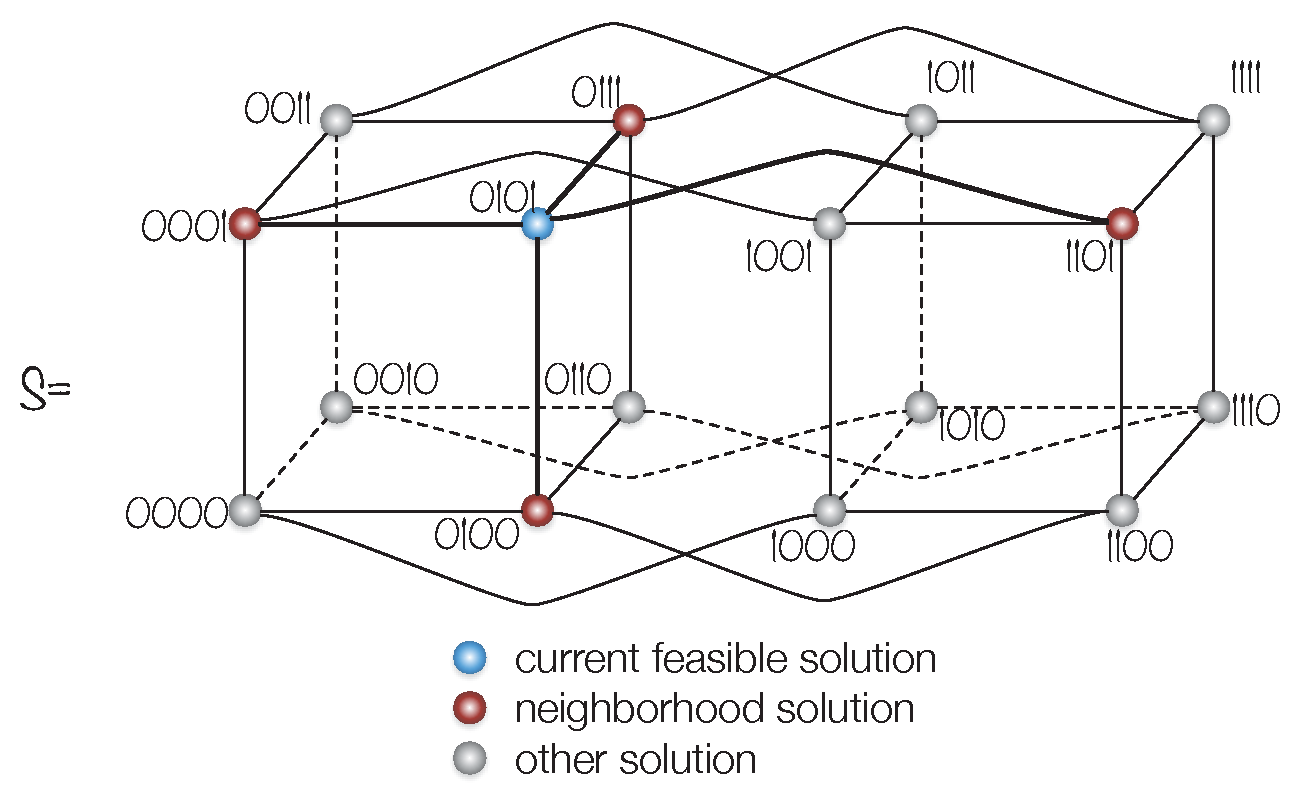
\includegraphics[width=4.0in]{paper-MPAR/hypercube}
\caption{超立方体解空间}
\label{fig:chap3_hypercube}
\end{figure}

停止规则是禁忌搜索中最重要的准则之一,其决定搜索过程停止的条件。在本算法中,停止规则如定义~\ref{def:stop_rule}所示。

\begin{definition}停止规则\\
停止规则 $\mathcal{E}$ 如下定义
\[
\mathcal{E}(\textbf{x}^{best})=\left\{
\begin{array}{cl}
true & \textnormal{if $p(\textbf{x}^{best})$ not improved after $\theta$ steps} \\
false & \textnormal{otherwise}
\end{array}\right.
\]
\label{def:stop_rule}
\end{definition}

如之前所述,评估函数$p$的值在搜索过程的每一次迭代中都被更新。如果当前解向量$\bm{x}^{now}$对应更好的评估函数值,即若有$p(\bm{x}^{now})>p(\bm{x}^{best})$,则用$\bm{x}^{now}$的值更新$\bm{x}^{best}$。然而,若当前记录的最优解对应的评估函数值$p(\bm{x}^{best})$在一定步数之内都未被更新,则意味着算法可能无法找到更好的解(在算法本身不被修改的前提下)。在这种情况下,搜索过程停止,当前最优解向量将作为返回值从算法返回。

禁忌表$\mathcal{T}$由两个主要元素组成,禁忌对象$\phi$和禁忌长度$\mathcal{L}(\phi)$。禁忌对象是禁忌搜索算法中实施禁忌的目标元素,可以定义为解向量的变化,或评估函数的变化。在本算法中,禁忌对象见定义~\ref{def:tabu_element}。

\begin{definition}禁忌对象\\
禁忌对象为解向量的变化,形式化定义如下
\[
\varphi:\textbf{x}\rightarrow\textbf{x'}
\]
有
\[
\textbf{x}=(x_1,\ldots,x_{i-1},x_i,x_{i+1},\ldots,x_n)~~(i\in [0,n])
\]
且
\[
\textbf{x'}=(x_1,\ldots,x_{i-1},y_i,x_{i+1},\ldots,x_n)~~(i\in [0,n], x_i\neq y_i)
\]
\label{def:tabu_element}
\end{definition}

事实上,禁忌对象是当前解向量在超立方体中对应的顶点向邻接顶点的迁移。正如\figurename~\ref{fig:chap3_hypercube}所示,从蓝色顶点(当前解)向红色顶点的迁移,即为禁忌对象。禁忌表中的禁忌长度如定义~\ref{def:tabu_length}。

\begin{definition}禁忌长度\\
禁忌长度由$\mathcal{L}(\varphi)$表示, 有
\[
\mathcal{L}(\varphi)=\lfloor T\rfloor
\]
T是服从正态分布的随机变量,有$T\sim N(\mu,\sigma^2)$, 且令
\[
\mu=\left\{
\begin{array}{ll}
\sqrt{n}[1+p(\textbf{x'})-p(\textbf{x})] & p(\textbf{x'})>p(\textbf{x}) \\
\sqrt{n} & \textnormal{otherwise}
\end{array}
\right.
\]
\label{def:tabu_length}
\end{definition}

在定义~\ref{def:tabu_element}中,禁忌长度设为对服从正态分布的随机变量$T$做下取整,其中正态分布的参数$\mu$保证了对于能让目标函数值变的更好的解向量,在统计意义上具有一个较长的禁忌长度。将禁忌长度设为一个随机数,而非常量,其意义在于向搜索算法中加上一定的随机因素,如同舍伍德算法一样。随机性能够帮助算法跳出一些无休止的循环,且能在算法输入被蓄意设定的情况下表现的更好。对于禁忌长度,值$T$与评估函数的变化程度$|p(\bm{x})-p(\bm{x'})|$具有一定关系。评估函数值发生变化具有两种情况;第一种情况下$p(\bm{x'})<p(\bm{x})$,意味着评估函数值到达了一个新的“山谷”;第二种情况下$p(\bm{x'})>p(\bm{x})$,意味着评估函数值爬上了一个比以往更高的“峰顶”。在第一种情况下,应将禁忌长度设的更大,从而让算法能够跳出当前的局部陷阱;对于第二种情况,应将禁忌长度设的更小,以免解向量移动的太远,再次掉入另一个“山谷”。定义~\ref{def:tabu_element}中的设定正好符合以上几点,此外对于正态分布参数$\mu$,有$\mu\in[\sqrt{n},2\sqrt{n}]$。

从定义~\ref{def:tabu_element}和定义~\ref{def:tabu_length}出发,算法禁忌表见定义~\ref{def:tabu_table}。

\begin{definition}禁忌表\\
禁忌表的结构如下 \\
\begin{center}
$\mathcal{T}$=
  \begin{tabular}{|c|c|cc|c|c|}
  \hline
   $1$ & $2$ & $\cdots$ & $\cdots$ & $n-1$ & $n$\\
   \hline
   $t_1$ & $t_2$ & $\cdots$ & $\cdots$ & $t_{n-1}$ & $t_n$ \\
    \hline
  \end{tabular} \\
\end{center}
假设禁忌对象为 $\varphi:\textbf{x}->\textbf{x'}$, 其更新规则如下
\[
\forall i, t_i=\left\{
\begin{array}{ll}
\mathcal{L}(\varphi) & \textnormal{if $|x_i-x'_i|=1$} \\
  0 & \textnormal{if}~t_i=0 \\
t_i-1 &  \textnormal{otherwise} \\
\end{array}
\right.
\]
\label{def:tabu_table}
\end{definition}

禁忌表$\mathcal{T}$设为一个$2\times n$的表,其中第一行代表禁忌对象中解向量的变化位置,第二行代表对于每个位置当前的禁忌步长。例如,设当前解向量发生变化,其对应的禁忌对象为$\phi:[0,1,0]\rightarrow[1,1,0]$,则应当按如下更新当前的禁忌表(其中$t_1,t_2,t_3>0$)
\begin{center}
\begin{tabular}{|c|c|c|}
\hline
1 & 2 & 3 \\
\hline
$t_1$ & $t_2$ & $t_3$ \\
\hline
\end{tabular} $\longrightarrow$
\begin{tabular}{|c|c|c|}
\hline
1 & 2 & 3 \\
\hline
$\mathcal{L}(\varphi)$ & $t_2-1$ & $t_3-1$ \\
\hline
\end{tabular}
\end{center}
对于算法的每一次更新操作,向量变化所对应的位置,在禁忌表中都会以$\mathcal{L}(\phi)$值更新,其它所有非零的表格元素都会做减1操作。任意位置,若其对应的禁忌步长不为0,则仅当禁忌步长降为0时,当前解向量才可从该位置向对应的相邻解向量迁移。

禁忌搜索中另一个重要的法则,即为特赦准则。特赦准则可以对禁忌表中特定的禁忌对象进行赦免,从而使其能被算法重新选取。特赦准则如定义~\ref{def:aspiration}

\begin{definition} 特赦准则\\
特赦准则如下定义
\begin{center}
\begin{tabular}{|c|}
\hline
对于 $\forall\bm{x}$, 若有 $p(\textbf{x})>p(\textbf{x}^{best})$ \\
则解向量 $\textbf{x}$ 可以作为下一步选择,即使其在禁忌表$\mathcal{T}$中被禁 \\
\hline
\end{tabular}
\end{center}
\label{def:aspiration}
\end{definition}

当所有的位置都在表$\mathcal{T}$中被禁时,当前解向量无法迁移到任何一个邻居向量。然而当某一个邻居向量所对应的评估函数值,优于当前所记录的最优值,则该向量会以特赦准则被解禁,即可以被算法选取。

\figurename~\ref{fig:chap3_example1}所示例子所对应的禁忌搜索过程,如\figurename~\ref{tab:chap3_tabu_search}。如同\tablename~\ref{tab:chap3_local_search}所示的局部搜索一样,消息源节点依然被选为$n_2$,且初始解向量为$[0,1,0]$。为了简化表述,在此,禁忌表长$\mathcal{L}$设定为常数$3$,而非定义中所述的随机量。此外,定义~\ref{def:stop_rule}中的$\theta$值设为$3$.

\begin{table*}[hbt]
  \caption{\figurename~\ref{fig:chap3_example1}例子对应的禁忌搜索过程}
  \resizebox{\textwidth}{!}{
  \begin{tabular}{|c|c|c|c|c|c|c|c|c|c|c|c|}
    \hline
    %empty 
    & \multicolumn{3}{c|}{current solution}
    & \multicolumn{3}{c|}{current best solution}
    & \multicolumn{1}{c|}{\multirow{2}{*}{tabu table $\mathcal{T}$}}
    & \multicolumn{4}{c|}{next options}
    \\    
    \cline{2-7}\cline{9-12}
    
    %empty 
    & $\textbf{x}^{now}$ & N & $P_{N,4}$ & $\textbf{x}^{best}$ & $N^{best}$ & $P_{N^{best},4}$ & & $\textbf{x}^{next}$ & N' & $P_{N',4}$ & status \\
    \hline
%    
    %%%%step 1
    \multicolumn{1}{|c|}{\multirow{3}{*}{\textbf{Step 1}}}
    &\multicolumn{1}{c|}{\multirow{3}{*}{$[0,1,0]$}}
    &\multicolumn{1}{c|}{\multirow{3}{*}{$\{n_2\}$}}
    &\multicolumn{1}{c|}{\multirow{3}{*}{$0.673$}}
    &\multicolumn{1}{c|}{\multirow{3}{*}{$[0,1,0]$}}
    &\multicolumn{1}{c|}{\multirow{3}{*}{$\{n_2\}$}}
    &\multicolumn{1}{c|}{\multirow{3}{*}{$0.673$}}
    &\multicolumn{1}{c|}{\multirow{3}{*}{$
                                                     \begin{tabular}{|c|c|c|}
                                                        \hline
                                                        1 & 2 & 3 \\
                                                        \hline
                                                        0 & 0 & 0 \\
                                                        \hline
                                                     \end{tabular}$}}
    &$[\underline{1},1,0]$ &$\{n_1,n_2\}$ & $0.670$ & choosable
    \\
    
    \multicolumn{1}{|c|}{}
    &\multicolumn{1}{c|}{}
    &\multicolumn{1}{c|}{}
    &\multicolumn{1}{c|}{}
    &\multicolumn{1}{c|}{}
    &\multicolumn{1}{c|}{}
    &\multicolumn{1}{c|}{}
    &\multicolumn{1}{c|}{}
    &$[0,\underline{0},0]$ & $\phi$ & $0$ & choosable
    \\
    
    \multicolumn{1}{|c|}{}
    &\multicolumn{1}{c|}{}
    &\multicolumn{1}{c|}{}
    &\multicolumn{1}{c|}{}
    &\multicolumn{1}{c|}{}
    &\multicolumn{1}{c|}{}
    &\multicolumn{1}{c|}{}
    &\multicolumn{1}{c|}{}
    &$[0,1,\underline{1}]$ & $\{n_2,n_3\}$ & $0.600$ & choosable
    \\
    \hline
    
    %%%%step 2
    \multicolumn{1}{|c|}{\multirow{3}{*}{\textbf{Step 2}}}
    &\multicolumn{1}{c|}{\multirow{3}{*}{$[1,1,0]$}}
    &\multicolumn{1}{c|}{\multirow{3}{*}{$\{n_1,n_2\}$}}
    &\multicolumn{1}{c|}{\multirow{3}{*}{$0.670$}}
    &\multicolumn{1}{c|}{\multirow{3}{*}{$[0,1,0]$}}
    &\multicolumn{1}{c|}{\multirow{3}{*}{$\{n_2\}$}}
    &\multicolumn{1}{c|}{\multirow{3}{*}{$0.673$}}
    &\multicolumn{1}{c|}{\multirow{3}{*}{$
                                                     \begin{tabular}{|c|c|c|}
                                                        \hline
                                                        1 & 2 & 3 \\
                                                        \hline
                                                        3 & 0 & 0 \\
                                                        \hline
                                                     \end{tabular}$}}
    &$[\underline{0},1,0]$ &$\{n_2\}$ & $0.673$ & tabu
    \\
    
    \multicolumn{1}{|c|}{}
    &\multicolumn{1}{c|}{}
    &\multicolumn{1}{c|}{}
    &\multicolumn{1}{c|}{}
    &\multicolumn{1}{c|}{}
    &\multicolumn{1}{c|}{}
    &\multicolumn{1}{c|}{}
    &\multicolumn{1}{c|}{}
    &$[0,\underline{0},0]$ & $\phi$ & $0$ & choosable
    \\
    
    \multicolumn{1}{|c|}{}
    &\multicolumn{1}{c|}{}
    &\multicolumn{1}{c|}{}
    &\multicolumn{1}{c|}{}
    &\multicolumn{1}{c|}{}
    &\multicolumn{1}{c|}{}
    &\multicolumn{1}{c|}{}
    &\multicolumn{1}{c|}{}
    &$[1,1,\underline{1}]$ & $\{n_1,n_2,n_3\}$ & $0.789$ & choosable
    \\

    \hline
    %%%%step 3
    \multicolumn{1}{|c|}{\multirow{3}{*}{\textbf{Step 3}}}
    &\multicolumn{1}{c|}{\multirow{3}{*}{$[1,1,1]$}}
    &\multicolumn{1}{c|}{\multirow{3}{*}{$\{n_1,n_2,n_3\}$}}
    &\multicolumn{1}{c|}{\multirow{3}{*}{$0.789$}}
    &\multicolumn{1}{c|}{\multirow{3}{*}{$[1,1,1]$}}
    &\multicolumn{1}{c|}{\multirow{3}{*}{$\{n_1,n_2,n_3\}$}}
    &\multicolumn{1}{c|}{\multirow{3}{*}{$0.789$}}
    &\multicolumn{1}{c|}{\multirow{3}{*}{$
                                                     \begin{tabular}{|c|c|c|}
                                                        \hline
                                                        1 & 2 & 3 \\
                                                        \hline
                                                        2 & 0 & 3 \\
                                                        \hline
                                                     \end{tabular}$}}
    &$[\underline{0},1,1]$ &$\{n_2,n_3\}$ & $0.600$ & tabu
    \\
    
    \multicolumn{1}{|c|}{}
    &\multicolumn{1}{c|}{}
    &\multicolumn{1}{c|}{}
    &\multicolumn{1}{c|}{}
    &\multicolumn{1}{c|}{}
    &\multicolumn{1}{c|}{}
    &\multicolumn{1}{c|}{}
    &\multicolumn{1}{c|}{}
    &$[1,\underline{0},1]$ & $\{n_1,n_3\}$ & $0.626$ & choosable
    \\
    
    \multicolumn{1}{|c|}{}
    &\multicolumn{1}{c|}{}
    &\multicolumn{1}{c|}{}
    &\multicolumn{1}{c|}{}
    &\multicolumn{1}{c|}{}
    &\multicolumn{1}{c|}{}
    &\multicolumn{1}{c|}{}
    &\multicolumn{1}{c|}{}
    &$[1,1,\underline{0}]$ & $\{n_1,n_2\}$ & $0.670$ & tabu
    \\

    \hline
    %%%%step 4
    \multicolumn{1}{|c|}{\multirow{3}{*}{\textbf{Step 4}}}
    &\multicolumn{1}{c|}{\multirow{3}{*}{$[1,0,1]$}}
    &\multicolumn{1}{c|}{\multirow{3}{*}{$\{n_1,n_3\}$}}
    &\multicolumn{1}{c|}{\multirow{3}{*}{$0.626$}}
    &\multicolumn{1}{c|}{\multirow{3}{*}{$[1,1,1]$}}
    &\multicolumn{1}{c|}{\multirow{3}{*}{$\{n_1,n_2,n_3\}$}}
    &\multicolumn{1}{c|}{\multirow{3}{*}{$0.789$}}
    &\multicolumn{1}{c|}{\multirow{3}{*}{$
                                                     \begin{tabular}{|c|c|c|}
                                                        \hline
                                                        1 & 2 & 3 \\
                                                        \hline
                                                        1 & 3 & 2 \\
                                                        \hline
                                                     \end{tabular}$}}
    &$[\underline{0},0,1]$ &$\{n_3\}$ & $0.291$ & tabu
    \\
    
    \multicolumn{1}{|c|}{}
    &\multicolumn{1}{c|}{}
    &\multicolumn{1}{c|}{}
    &\multicolumn{1}{c|}{}
    &\multicolumn{1}{c|}{}
    &\multicolumn{1}{c|}{}
    &\multicolumn{1}{c|}{}
    &\multicolumn{1}{c|}{}
    &$[1,\underline{1},1]$ & $\{n_1,n_2,n_3\}$ & $0.789$ & tabu
    \\
    
    \multicolumn{1}{|c|}{}
    &\multicolumn{1}{c|}{}
    &\multicolumn{1}{c|}{}
    &\multicolumn{1}{c|}{}
    &\multicolumn{1}{c|}{}
    &\multicolumn{1}{c|}{}
    &\multicolumn{1}{c|}{}
    &\multicolumn{1}{c|}{}
    &$[1,0,\underline{0}]$ & $\{n_1\}$ & $0.430$ & tabu
    \\
    
    \hline
    %%%%step 5
    \multicolumn{1}{|c|}{\multirow{3}{*}{\textbf{Step 5}}}
    &\multicolumn{1}{c|}{\multirow{3}{*}{$[1,0,1]$}}
    &\multicolumn{1}{c|}{\multirow{3}{*}{$\{n_1,n_3\}$}}
    &\multicolumn{1}{c|}{\multirow{3}{*}{$0.626$}}
    &\multicolumn{1}{c|}{\multirow{3}{*}{$[1,1,1]$}}
    &\multicolumn{1}{c|}{\multirow{3}{*}{$\{n_1,n_2,n_3\}$}}
    &\multicolumn{1}{c|}{\multirow{3}{*}{$0.789$}}
    &\multicolumn{1}{c|}{\multirow{3}{*}{$
                                                     \begin{tabular}{|c|c|c|}
                                                        \hline
                                                        1 & 2 & 3 \\
                                                        \hline
                                                        0 & 2 & 1 \\
                                                        \hline
                                                     \end{tabular}$}}
    &$[\underline{0},0,1]$ &$\{n_3\}$ & $0.291$ & choosable
    \\
    
    \multicolumn{1}{|c|}{}
    &\multicolumn{1}{c|}{}
    &\multicolumn{1}{c|}{}
    &\multicolumn{1}{c|}{}
    &\multicolumn{1}{c|}{}
    &\multicolumn{1}{c|}{}
    &\multicolumn{1}{c|}{}
    &\multicolumn{1}{c|}{}
    &$[1,\underline{1},1]$ & $\{n_1,n_2,n_3\}$ & $0.789$ & tabu
    \\
    
    \multicolumn{1}{|c|}{}
    &\multicolumn{1}{c|}{}
    &\multicolumn{1}{c|}{}
    &\multicolumn{1}{c|}{}
    &\multicolumn{1}{c|}{}
    &\multicolumn{1}{c|}{}
    &\multicolumn{1}{c|}{}
    &\multicolumn{1}{c|}{}
    &$[1,0,\underline{0}]$ & $\{n_1\}$ & $0.430$ & tabu
    \\
    
    \hline
    %%%%stop
    \multicolumn{1}{|c|}{\multirow{3}{*}{\textbf{Stop}}}
    &\multicolumn{1}{c|}{\multirow{3}{*}{$[1,1,1]$}}
    &\multicolumn{1}{c|}{\multirow{3}{*}{$\{n_1,n_2,n_3\}$}}
    &\multicolumn{1}{c|}{\multirow{3}{*}{$0.789$}}
    &\multicolumn{1}{c|}{\multirow{3}{*}{---}}
    &\multicolumn{1}{c|}{\multirow{3}{*}{---}}
    &\multicolumn{1}{c|}{\multirow{3}{*}{---}}
    &\multicolumn{1}{c|}{\multirow{3}{*}{---}}
    &\multicolumn{1}{c|}{\multirow{3}{*}{---}} 
    &\multicolumn{1}{c|}{\multirow{3}{*}{---}} 
    &\multicolumn{1}{c|}{\multirow{3}{*}{---}}  
    &\multicolumn{1}{c|}{\multirow{3}{*}{---}}
    \\
    
    \multicolumn{1}{|c|}{}
    &\multicolumn{1}{c|}{}
    &\multicolumn{1}{c|}{}
    &\multicolumn{1}{c|}{}
    &\multicolumn{1}{c|}{}
    &\multicolumn{1}{c|}{}
    &\multicolumn{1}{c|}{}
    &\multicolumn{1}{c|}{}
    & &  &  &
    \\
    
    \multicolumn{1}{|c|}{}
    &\multicolumn{1}{c|}{}
    &\multicolumn{1}{c|}{}
    &\multicolumn{1}{c|}{}
    &\multicolumn{1}{c|}{}
    &\multicolumn{1}{c|}{}
    &\multicolumn{1}{c|}{}
    &\multicolumn{1}{c|}{}
    & &  &  &
    \\    
    \hline    
  \end{tabular}}
  \label{tab:chap3_tabu_search}
\end{table*}

在Step 1中,禁忌表$\mathcal{T}$初始化为空,对于当前解向量,其所有的邻居解向量都可选。依算法\ref{alg:chap3_framework}第5行,选择能使评估函数取最大值的解向量$[1,1,0]$。在Step 2中,解向量第一个位置在表中被禁,故下一个解向量只能在$[0,0,0]$及$[1,1,1]$中选择。搜索过程一直进行到Step 5,其中最优解在$\theta=3$步之后还未更新,触发停止规则,算法终止。纵览整个过程,与\tablename~\ref{tab:chap3_local_search}所述局部搜索过程相比,算法可以成功跳出局部最优陷阱。

\section{最优化路由算法}
\label{chap3:最优化路由算法}

本节给出有关路由过程的细节。在本节中,提出两个路由算法,基于局部搜索的Local-MPAR和基于禁忌搜索的Tabu-MPAR。在Local-MPAR中,对任一节点而言,其它节点的$\lambda$值仅当该节点与其接触时获取;在Tabu-MPAR中,假设每个节点都知道其它所有节点对应的$\lambda$值。

在本章中,算法过程的解释是针对单一消息而言的(该消息在网络中可以具有一份或者多份拷贝)。为了进一步解释路由算法,本章参照文献\upcite{Vahdat2000}所提出的传染病路由算法的概念——将消息看做传播的病毒。由此,节点间一次成功的消息传输(复制)可被看做一次感染。上述讨论中,不包括消息的投递过程,即假设当$n_a$感染$n_b$时,$n_b$不为消息的目的节点。以此出发,可以将网络中的节点状态划分为三类(皆只针对某一消息而言)。

\begin{itemize}
\item \textbf{被感染节点}\\
被感染节点持有一条或者几条该消息的拷贝,然而被感染节点不具备传染性,即无法传染其他纯净节点。

\item \textbf{纯净节点}\\
纯净节点不持有消息的任意拷贝,可以被任意传染节点感染。

\item \textbf{传染节点}\\
传染节点是一类特殊的被感染节点,其可以传染其它纯净节点。
\end{itemize}

从传染状态可以迁移到被感染状态;换言之,节点将仍然持有该条消息,然而无法将该消息复制给其它节点。纯净状态也可以迁移到被感染状态或传染状态;当此类状态迁移发生,则说明该节点接受了消息。为了进一步解释这类状态迁移,下面将参照Epidemic算法\upcite{Vahdat2000}及SprayAndWait算法\upcite{Spyropoulos2005}进行说明。

在Epidemic路由算法中,有两类状态节点,纯净节点和传染节点。消息副本的分发过程在所有纯净节点都被感染,都迁移至传染状态时结束。SprayAndWait路由算法中,节点可以处于以上三种状态中的任意一种。在Source SprayAndWait中,网络中只有一个传染节点,在Binary SprayAndWait中,传染节点允许有多个,但是其最大数量被限制为一个固定数目。当网络中不在有传染节点时,消息分发过程结束。

事实上,这几类节点几乎存在于所有的机会网络路由算法中。特别地,Epidemic及SprayAndWait是两类具有代表性的零知识依赖路由算法。对于其它路由算法,其消息副本分发过程亦可按照此类节点状态划分方法进行分类,从而可视作Epidemic及SprayAndWait算法的改进。在介绍Local-MPAR及Tabu-MPAR之前,先提出本章关于路由的三个公设。

\begin{postulation}
\label{post:replication}
对任意节点$n_a$而言,$n_a$从$n_b$接受某条消息,当且仅当其不持有该消息的任意拷贝。
\end{postulation}

\begin{postulation}
\label{post:deletion}
当消息的time-to-live到期时,从缓存中清除该消息的行为叫做丢弃;因节点状态迁移而清除缓存消息的行为,叫做删除。
\end{postulation}

\begin{postulation}
持有某条消息或该条消息任意拷贝的某一组节点,记为$N$,由所有传染节点及被感染节点组成。
\end{postulation}

Local-MPAR及Tabu-MPAR中的状态迁移图,如\figurename~\ref{fig:chap3_states2}及\figurename~\ref{fig:chap3_states3}所示,有如下定理。

\begin{figure}[!t]
\centering
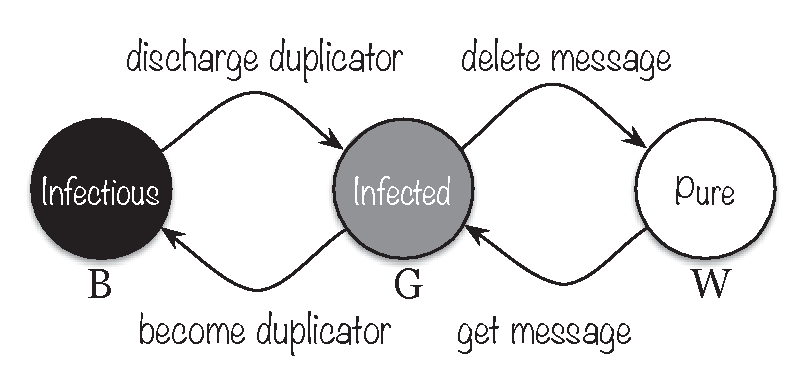
\includegraphics[width=3in]{paper-MPAR/states2}
\caption{Local-MPAR节点状态迁移图.}
\label{fig:chap3_states2}
\end{figure}

\begin{figure}[!tb]
\centering
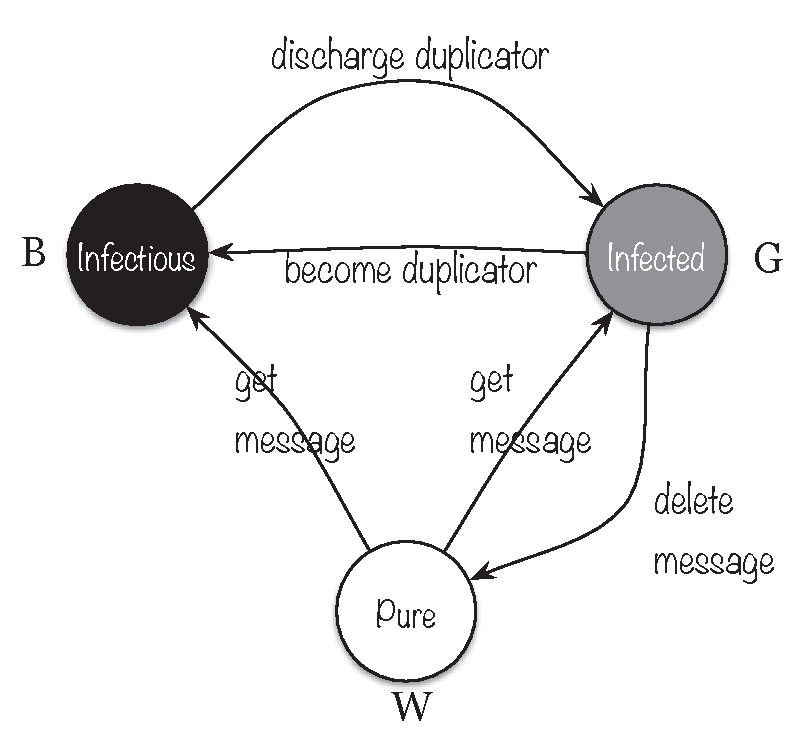
\includegraphics[width=3in]{paper-MPAR/states3}
\caption{Tabu-MPAR节点状态迁移图.}
\label{fig:chap3_states3}
\end{figure}


\begin{table*}[hbt]
\centering
  \caption{Local-MPAR中的节点状态迁移}
  \label{tab:chap3_Local-MPAR}
  \resizebox{\textwidth}{!}{
  \begin{tabular}{|c|c|c|c|c|}
  \hline

   &\multicolumn{4}{c|}{\textbf{state of $n_{b}$}}
   \\
   \hline
    \multicolumn{1}{|c|}{\multirow{9}{*}{\textbf{state of $n_{a}$}}}
   &
   & \textbf{B}
   & \textbf{G}
   & \textbf{W}
   \\
   \cline{2-5}
   & \textbf{B}
   & \multicolumn{1}{c:}{---}
   & \multicolumn{1}{c:}{B
     $\rightarrow\left\{
     \begin{array}{ll} 
      \textnormal{G} & \textnormal{if}~\textnormal{G}\rightarrow\textnormal{B happens in }n_b\\
      \textnormal{B} & \textnormal{else}
     \end{array}\right.
     $}
   & B
   \\
   \cline{2-2}\cdashline{3-5}
   & \textbf{G}
   & \multicolumn{1}{c:}{G
     $\rightarrow\left\{
     \begin{array}{ll}
      \textnormal{W} & \textnormal{if}~P_{N-\{n_a\},d}>P_{N,d} \\
      \textnormal{B} & \textnormal{if}~P_{N-\{n_a\}}\leq P_{N,d}~\textnormal{and}~E[D_a]<E[D_b] \\
      \textnormal{G} & \textnormal{else}
     \end{array}\right.
     $}
   & \multicolumn{1}{c:}{G}
   & G
   \\
   \cline{2-2}\cdashline{3-5}
   & \textbf{W}
   & \multicolumn{1}{c:}{W
     $\rightarrow\left\{
     \begin{array}{ll}
      \textnormal{G} & \textnormal{if}~P_{N\bigcup\{n_b\},d}>P_{N,d} \\
      \textnormal{W} & \textnormal{else}
     \end{array}\right.
     $}
   & \multicolumn{1}{c:}{W}
   & W
   \\
  \hline
  \end{tabular}}
\end{table*}

\begin{table*}[hbt]
\centering
  \caption{Tabu-MPAR中的节点状态迁移}
  \label{tab:chap3_Tabu-MPAR}
  \resizebox{\textwidth}{!}{
  \begin{tabular}{|c|c|c|c|c|}
  \hline

   &\multicolumn{4}{c|}{\textbf{state of $n_{b}$}}
   \\
   \hline
    \multicolumn{1}{|c|}{\multirow{9}{*}{\textbf{state of $n_{a}$}}}
   &
   & \textbf{B}
   & \textbf{G}
   & \textbf{W}
   \\
   \cline{2-5}
   & \textbf{B}
   & \multicolumn{1}{c:}{B}
   & \multicolumn{1}{c:}{
       \begin{tabular}{c}
     $B\rightarrow B|G$\\
     \textit{(depends on the tickets left in $n_a$} \\
     \textit{after allocating to $n_b$)} \\
     \end{tabular}
   }
   & 
    \begin{tabular}{c}
     $B\rightarrow B|G$\\
     \textit{(depends on the} \\
     \textit{tickets left in $n_a$} \\
     \textit{after allocating to $n_b$)} \\
     \end{tabular}
   \\
   \cline{2-2}\cdashline{3-5}
   & \textbf{G}
   & \multicolumn{1}{c:}{
   \begin{tabular}{c}
     $G\rightarrow B|G$\\
     \textit{(depends on the} \\
     \textit{tickets left in $n_a$} \\
     \textit{after allocating to $n_b$)} \\
     \end{tabular}
   }
   & \multicolumn{1}{c:}{G}
   & G
    $\rightarrow\left\{
     \begin{array}{ll}
      W & \textnormal{if}~n_a\notin N_{opt}~\textnormal{and}~n_b\in N_{opt}\\
      G & \textnormal{else}
     \end{array}\right.
    $
   \\
   \cline{2-2}\cdashline{3-5}
   & \textbf{W}
   & \multicolumn{1}{c:}{
     \begin{tabular}{c}
     $W\rightarrow B|G$\\
     \textit{(depends on the} \\
     \textit{tickets left in $n_a$} \\
     \textit{after allocating to $n_b$)} \\
     \end{tabular}
     }
   & \multicolumn{1}{c:}{W
    $\rightarrow\left\{
    \begin{array}{ll}
     \textnormal{G} & \textnormal{if}~n_a\in N_{opt}~\textnormal{and}~n_b\notin N_{opt}\\
     \textnormal{W} & \textnormal{else}
    \end{array}\right.
    $
   }
   & W
   \\
  \hline
  \end{tabular}}
\end{table*}

\begin{theorem}
\label{theorem:replication_deletion}
%The replication operation is corresponding to the transition from W to G and deletion operation to the transition from G to W.
对应\tablename~\ref{tab:chap3_Tabu-MPAR}中的状态迁移,复制操作对应于$W\rightarrow G$,删除操作对应于$G\rightarrow W$。
\end{theorem}
\begin{proof}
从三种状态的定义可知,持有消息的节点,位于状态$B$或$G$,未持有消息的节点,对应于状态$W$。由于$B$与$W$之间无直接迁移路径,状态$B$只能经过状态$G$迁移至$W$,反之亦然。从公设~\ref{post:replication}可知,复制操作对应于状态迁移$W\rightarrow B$,其中包含迁移$W\rightarrow G$。从公设~\ref{post:deletion}可知,删除操作对应于$B\rightarrow W$,即有$G\rightarrow W$。\\
证毕
\end{proof}


\subsection{Local-MPAR:基于局部搜索的路由算法}

在Local-MPAR算法中,节点可以处于三种状态中的任一状态。然而,对于每一条从源节点产生的消息而言,只允许网络中存在不超过一个传染节点。Local-MPAR的基本思想,即是动态调整集合$N$,从而最大化预测投递概率$P_{N,d}$。

算法~\ref{alg:chap3_Local-MPAR}~阐述了Local-MPAR算法的过程。在Local-MPAR中共有三种状态,在初始状态时,源节点$n_s$产生了消息$M$,于是其状态被设为传染状态。相应地,集合$N$被初始化为只包含源节点$n_s$。对于集合$N$,有如下公设。

\begin{postulation}
\label{post:N}
在Local-MPAR中, 节点集合$N$总是被传染节点维护。
\end{postulation}

算法~\ref{alg:chap3_Local-MPAR}~中整个路由过程可以被视作动态调整集合$N$的过程,如Routing Stage所示。该Stage的关键操作,即是让每一个节点完成\tablename~\ref{tab:chap3_Local-MPAR}中的状态转换。为简单起见,称表中行B列G的位置为BG。从\tablename~\ref{tab:chap3_Local-MPAR}可以看出,对于任意两个相遇节点$n_a$及$n_b$,状态迁移仅发生在$n_a$和$n_b$至少有一个处于B状态时。BB中无行为发生,其原因是在Local-MPAR中,对于某一条消息而言,不可能有两个节点同时处于B状态。


\begin{algorithm}[tbp] %算法的开始
\renewcommand{\algorithmicensure}{\textbf{Initial Stage:}}
\caption{Local-MPAR Algorithm.} %算法的标题
\label{alg:chap3_Local-MPAR} %给算法一个标签,这样方便在文中对算法的引用
\begin{algorithmic}[1] %这个1 表示每一行都显示数字
\ENSURE
\STATE $n_s$ generates message $M$
\STATE $n_s.state\leftarrow$\textbf{B}
\STATE $N\leftarrow\{n_s\}$
\end{algorithmic} %这个1 表示每一行都显示数字
\begin{algorithmic}[1] %这个1 表示每一行都显示数字
\renewcommand{\algorithmicensure}{\textbf{Routing Stage:}}
\ENSURE
\FOR{any pair of $n_a$ and $n_b$}
    \IF{$n_a$ and $n_b$ encounter}
        \STATE finish the state transition according to \tablename~\ref{tab:chap3_Local-MPAR}
        \STATE update $N$
    \ENDIF
\ENDFOR
\end{algorithmic}
\begin{algorithmic}[1]
\renewcommand{\algorithmicensure}{\textbf{End Stage:}}
\ENSURE
\STATE $M$ is delivered
\end{algorithmic}
\end{algorithm}

\begin{lemma}
\label{lemma:infectious}
%The replication or deletion of message happens only if one of the encountered two nodes is in infectious state.
消息的复制过程或删除过程,仅当相遇的两个节点中其中一个为传染节点时,才会发生。
\end{lemma}
\begin{proof}
直接由 \tablename~\ref{tab:chap3_Local-MPAR}得出。\\
证毕
\end{proof}

\begin{theorem} 
%The routing stage of Local-MPAR is a local search process in the solution space $\mathcal{S}$.
Local-MPAR的路由阶段,即在解空间$\mathcal{S}$中做局部搜索。
\end{theorem}
\begin{proof}
%From postulation~4, we know that the node set $N$ is updated only in infectious node. Lemma~1 directly shows that any happened replication or deletion operation can be informed to the infectious node immediately, so that $N$ would be updated in time. Either a replication or deletion operation just causes 1 replicas difference in the network, thus only adding or removing one element in the set $N$, which indeed transfers the correspondent solution vector to one of its neighborhoods $\mathcal{N}(N)$. We can see from \tablename~4 that N would not vary if and only if $\forall N'\in\mathcal{N}(N), P_{N',d}\leq P_{N,d}$, i.e.,  if and only if the solution reaches the local optimum.
从公设~\ref{post:N}可知,节点集合$N$只会在传染节点中被更新。引理~\ref{lemma:infectious}直接可得,任何复制或删除操作可以立即被传染节点所知,即集合$N$可被及时更新。复制操作或删除操作,其只会引起网络中一份拷贝的数量差异,因此仅仅会从集合$N$中删除或增加一个元素,其本质即是将当前解向量迁移至其某一邻居解向量。从\tablename~\ref{tab:chap3_Local-MPAR}可知,$N$当且仅当$\forall N'\in\mathcal{N}(N), P_{N',d}\leq P_{N,d}$才不会再改变;即当且仅当解向量到达局部最优时,算法停止。\\
证毕
\end{proof}

另一个需要解释的问题是,既然Local-MPAR中只存在一个传染节点,那么该节点应当如何选取?其选取的基本准则,即是基于公式~(\ref{eq:delay})中对节点移动到下一个位置的延迟时间的预测。在\tablename~\ref{tab:chap3_Local-MPAR}中GB位置,当无需将$n_a$从状态G迁移至状态W时,应当考虑是否改变$n_a$为传染节点。若$E[D_a]$的值小于$E[D_b]$,则认为$n_a$更适合担当消息复制者,因为它具有更低的移动到下一位置的期望时延,意味着更多的传输机会。反之,若将消息复制权交给$n_b$,$n_b$将发生G$\rightarrow$B迁移,对称地,$n_a$将发生B$\rightarrow$G迁移。这样网络中仍然只保持有仅一个传染节点。

\figurename~\ref{fig:chap3_example1}中例子所示的Local-MPAR路由过程,如\figurename~\ref{fig:chap3_local_rt}所示。在时间$t_1$,节点$n_2$产生目的节点为$n_4$的消息。从时间$t_2$到$t_3$,由于集合$\{n_1,n_2\}$及集合$\{n_2,n_3\}$所对应的投递率都要小于集合$\{n_2\}$,$n_2$不会向$n_1$及$n_3$复制消息。最优集合$N_{opt}=\{n_1,n_2,n_3\}$所对应的投递概率,要比$\{n_2\}$所对应的投递概率大,然而,由于Local-MPAR算法无法跳出局部最优,故$N$无法变为$N_{opt}$。

\begin{figure}
\centering
\subfigure[Time $t_1$\label{local_rt1}]
{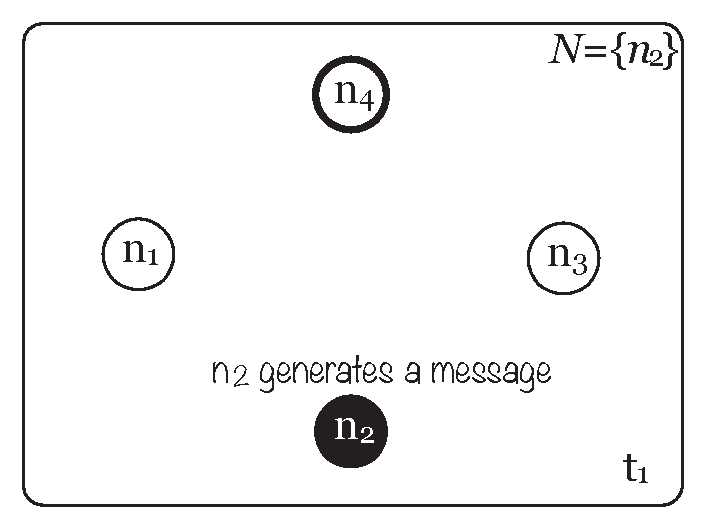
\includegraphics[width=0.45\linewidth]{paper-MPAR/local_rt1}}
\subfigure[Time $t_2$\label{local_rt2}]
{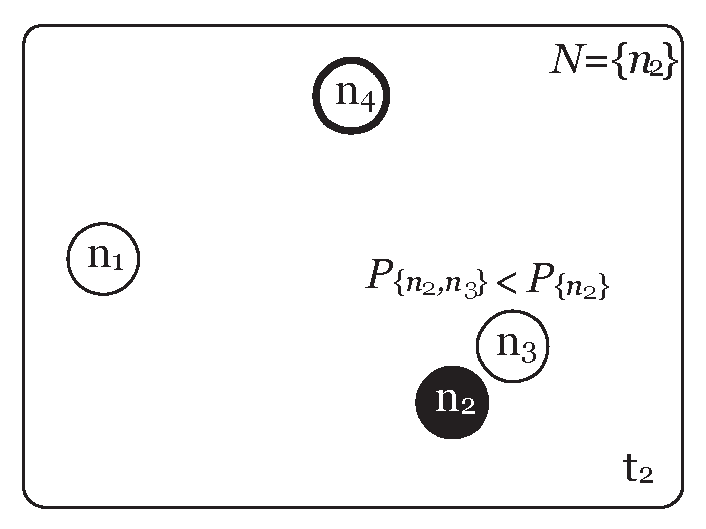
\includegraphics[width=0.45\linewidth]{paper-MPAR/local_rt2}} \\
\subfigure[Time $t_3$\label{local_rt3}]
{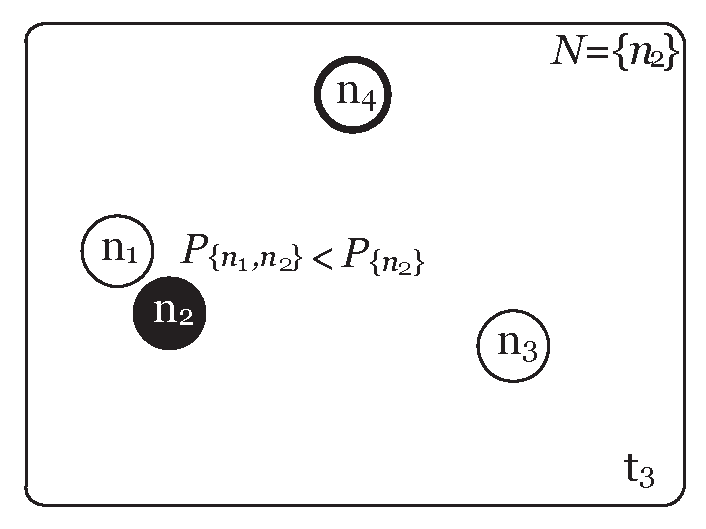
\includegraphics[width=0.45\linewidth]{paper-MPAR/local_rt3}}
\subfigure[Time $t_4$\label{local_rt4}]
{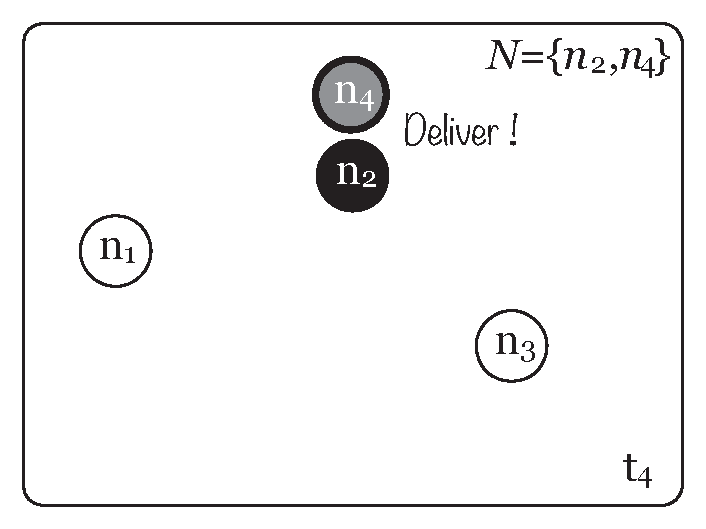
\includegraphics[width=0.45\linewidth]{paper-MPAR/local_rt4}}
\caption{Local-MPAR路由过程.}
\label{fig:chap3_local_rt}
\end{figure}

\subsection{Tabu-MPAR:基于禁忌搜索的路由算法}

在Tabu-MPAR算法中,与Local-MPAR相同,每个节点都有三个状态。如同SprayAndWait算法,允许网络中存在多于一个但有最大数目限制的传染节点。

Tabu-MPAR路由算法如算法~\ref{alg:chap3_Tabu-MPAR}所示。如同Local-MPAR, Tabu-MPAR算法亦分为三个阶段。在初始节点,当源节点$n_s$产生消息$M$时,节点$n_s$的状态被设为B,如行1--2所示。节点集合$N_{opt}$在源节点中计算,此外,对于每一条产生的消息,都对应有一个网络中该消息的最大副本数量,该值设为$|N_{opt}|$。每个节点对于每条消息,维护有一个计数变量,用以指明当前该节点持有该消息的拷贝数目。节点处于状态B,当且仅当其消息计数变量大于1\footnote{严格来讲,该节点是针对该条消息处于状态B,对于其它消息而言,该节点的状态也可能为W或者G。}.持有消息的计数变量为1的节点,处于状态G,不持有该消息的节点,皆处于状态P。

算法~\ref{alg:chap3_Tabu-MPAR}的第二阶段即是Tabu-MPAR的路由过程。与Local-MPAR相比,有两个不同点。首先,无需在路由过程中更新$N_{opt}$,因为其已在源节点$n_s$中被计算出来,并写入消息的头部。其次,当任意两个节点$n_a$及$n_b$相遇时,将在状态转换之前重新分配对应的消息计数变量。分配策略基于$E[D_a]$及$E[D_b]$的值,如行3及行4所示。具有更小$E[D]$值的节点,将被分配更多数目的消息拷贝。行5--10保证了变量$a$和$b$都是位于$1$和$L-1$之间的整数。由此可定义Tabu-MPAR的状态转换规则,如\tablename~\ref{tab:chap3_Tabu-MPAR}。除了表中对角线位置以外,其它表位置中都可能发生对应的状态迁移。事实上,当节点$n_a$发生GB位置的状态迁移时,节点$n_b$也同时发生BG位置的状态迁移,反之亦然。该规则也适用于WB,BW及WG,GW。故表\tablename~\ref{tab:chap3_Tabu-MPAR}可以看做一个$3\times 3$的对称矩阵。Tabu-MPAR路由过程如\figurename~\ref{fig:chap3_tabu_rt}所示。

\begin{algorithm}[htbp] %算法的开始
\renewcommand{\algorithmicensure}{\textbf{Initial Stage:}}
\caption{Tabu-MPAR Algorithm.} %算法的标题
\label{alg:chap3_Tabu-MPAR} %给算法一个标签,这样方便在文中对算法的引用
\begin{algorithmic}[1] %这个1 表示每一行都显示数字
\ENSURE
\STATE $n_s$ generates message $M$
\STATE $n_s.state\leftarrow$\textbf{B}
\STATE $n_s$ computes $N_{opt}$ by tabu search and saves it in $M$
\STATE $n_s.tickets\leftarrow |N_{opt}|$
\end{algorithmic} %这个1 表示每一行都显示数字
\begin{algorithmic}[1] %这个1 表示每一行都显示数字
\renewcommand{\algorithmicensure}{\textbf{Routing Stage:}}
\ENSURE
\FOR{any pair of $n_a$ and $n_b$}
    \IF{$n_a$ and $n_b$ encounter}
        \STATE $a=\frac{E[D_b]}{E[D_a]+E[D_b]}\cdot |N_{opt}|$
        \STATE $b=\frac{E[D_a]}{E[D_a]+E[D_b]}\cdot |N_{opt}|$
        \IF{$a<1$}
            \STATE $n_a.tickets=\lceil a \rceil$
            \STATE $n_b.tickets=\lfloor b \rfloor$
        \ELSE
            \STATE $n_a.tickets=\lfloor a \rfloor$
            \STATE $n_b.tickets=\lceil b \rceil$
        \ENDIF
        \STATE finish the state transition according to \tablename~\ref{tab:chap3_Tabu-MPAR}
    \ENDIF
\ENDFOR
\end{algorithmic}
\begin{algorithmic}[1]
\renewcommand{\algorithmicensure}{\textbf{End Stage:}}
\ENSURE
\STATE $M$ is delivered
\end{algorithmic}
\end{algorithm}

\begin{figure}
\centering
\subfigure[Time $t_1$\label{tabu_rt1}]
{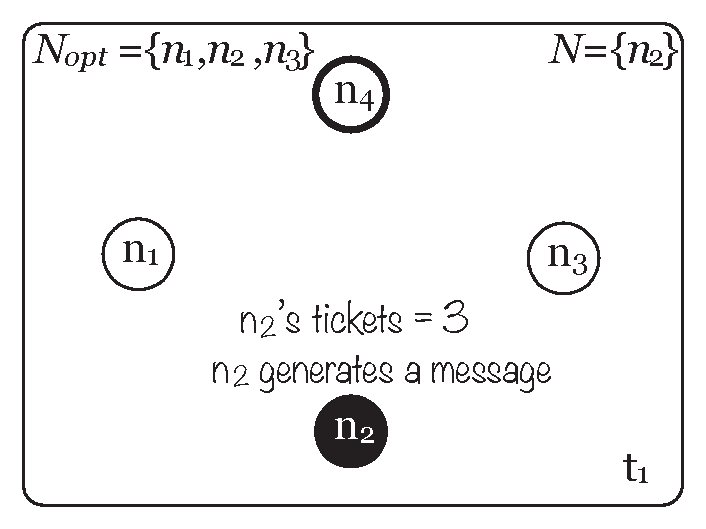
\includegraphics[width=0.45\linewidth]{paper-MPAR/tabu_rt1}}
\subfigure[Time $t_2$\label{tabu_rt2}]
{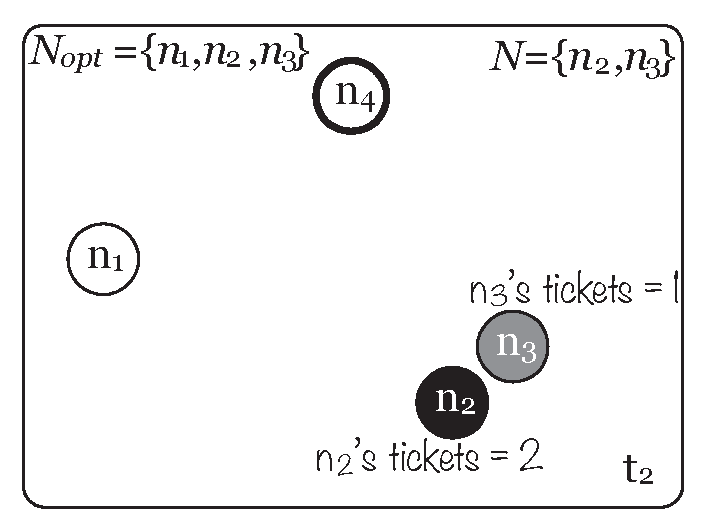
\includegraphics[width=0.45\linewidth]{paper-MPAR/tabu_rt2}} \\
\subfigure[Time $t_3$\label{tabu_rt3}]
{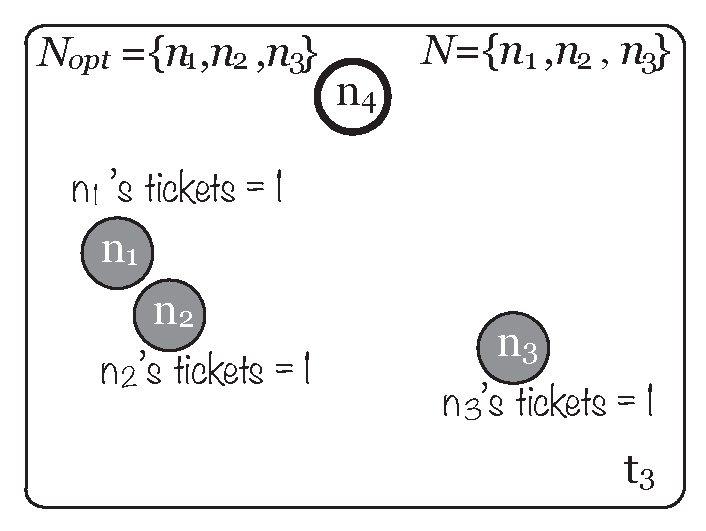
\includegraphics[width=0.45\linewidth]{paper-MPAR/tabu_rt3}}
\subfigure[Time $t_4$\label{tabu_rt4}]
{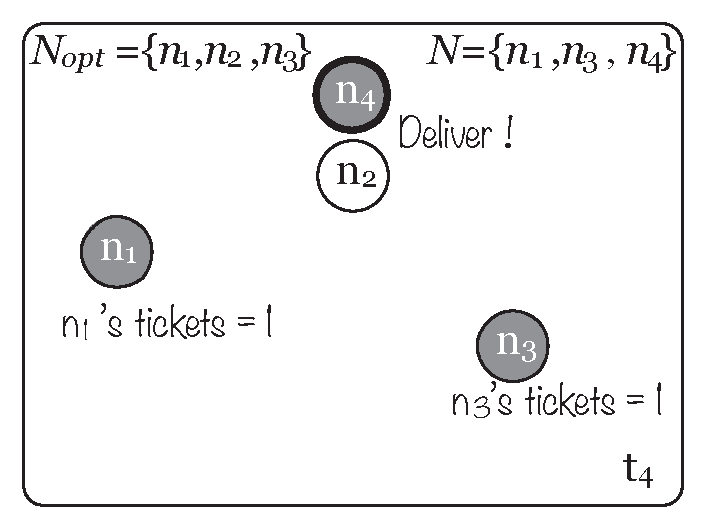
\includegraphics[width=0.45\linewidth]{paper-MPAR/tabu_rt4}}
\caption{Tabu-MPAR路由过程.}
\label{fig:chap3_tabu_rt}
\end{figure}

下面证明Tabu-MPAR的路由过程即对应$N$变为最优集合$N_{opt}$的过程。

\begin{lemma}
$N=N_{opt}$当且仅当网络中不存在传染节点时发生,即所有属于集合$N$中的节点,都处于状态G。
\label{lemma:no_infectious}
\end{lemma}
\begin{proof}
由于网络中某条消息最大副本数量为$|N_{opt}|$,若存在传染节点$n_a$,则其对应的拷贝数量至少为2,故其它节点一共所具有的拷贝数量不会超过$|N_{opt}|-2$。因此,持有该消息的所有节点的数目,至多为$|N_{opt}|-1$个,故其必要性成立。若持有该消息的节点集合为$|N_{opt}|$,则该条消息在网络中已达到其最大可能副本数量$|N_{opt}|$。在此情形下,每个节点所持有该消息的拷贝数目为1份。根据Tabu-MPAR节点状态的定义,集合$|N_{opt}|$中所有节点此时都处于被感染状态,即状态G;其它所有节点都为纯净节点,即处于状态W。此时,网络中无传染节点,故充分性成立。\\
证毕
\end{proof}



\begin{lemma}
若集合$N$变为$N_{opt}$,则不会再改变。
\label{lemma:change}
\end{lemma}
\begin{proof}
从引理~\ref{lemma:no_infectious}可知,若$N$变为$N_{opt}$,则所有$N$中的节点都处于状态G,且网络中所有的纯净节点都不在$N$中。由于网络中没有位于B状态的节点,状态迁移$B\rightarrow G$不会发生。对于状态迁移$G\rightarrow B$,若其发生,则一定伴随状态迁移$G\rightarrow W$发生;然而其只可能在处于$G$状态的节点不属于$|N_{opt}|$时发生,与题设矛盾。故集合$N$中所有节点的状态不会发生改变。\\
证毕
\end{proof}

\begin{theorem}
依\tablename~\ref{tab:chap3_Tabu-MPAR}中状态转移规则能够使集合$N$变为$N_{opt}$.
\end{theorem}
\begin{proof}
状态迁移B$\rightarrow$G不会使集合$N$发生改变。从算法~\ref{alg:chap3_Tabu-MPAR}4--10行可知,所有节点重新分配后的副本数目至少为1,即若有足够多的节点接触机会,则网络中所有处于B状态的节点最终都会变为状态G。考虑状态迁移W$\rightarrow$G及G$\rightarrow$W,其转换规则即符合$N_{opt}$。结合引理~\ref{lemma:no_infectious}及引理~\ref{lemma:change}即可证得本定理。\\
证毕
\end{proof}


\section{仿真实验及分析}
\label{chap3:仿真实验}

在本节中,基于机会网络仿真器(Opportunistic Network Environment, ONE)\upcite{Keranen2009},对MPAR算法进行仿真,并进行性能评估比较。节点移动模型采用\upcite{Ekman:2008fp}提出的Working Day Movement (WDM)模型,地图设为Manhattan Blocks。WDM模型分层结合了许多子节点移动模型。此外,一些常见的移动模型相关元素,如家,办公室,夜晚活动及不同的交通工具(如电车,私家车等)也在WDM中设定,用以捕捉人类社会相关属性。办公室模型(office sub-model)产生一种围绕办公桌的星形移动轨迹,相关的办公室人员按此轨迹进行移动。家模型(home sub-model)即是使人员在某个定点固定下自身位置,不做移动。夜晚活动模型(evening activity sub-model)反映了具有朋友关系的人群在工作后的活动,其使节点在街道上服从随机走方式移动。Manhattan Community模型将节点路径限制在街道上。Manhattan Community模型包含一组呈矩阵状的小格,如\figurename~\ref{fig:chap3_manhattan}。

\begin{figure}[!t]
\centering
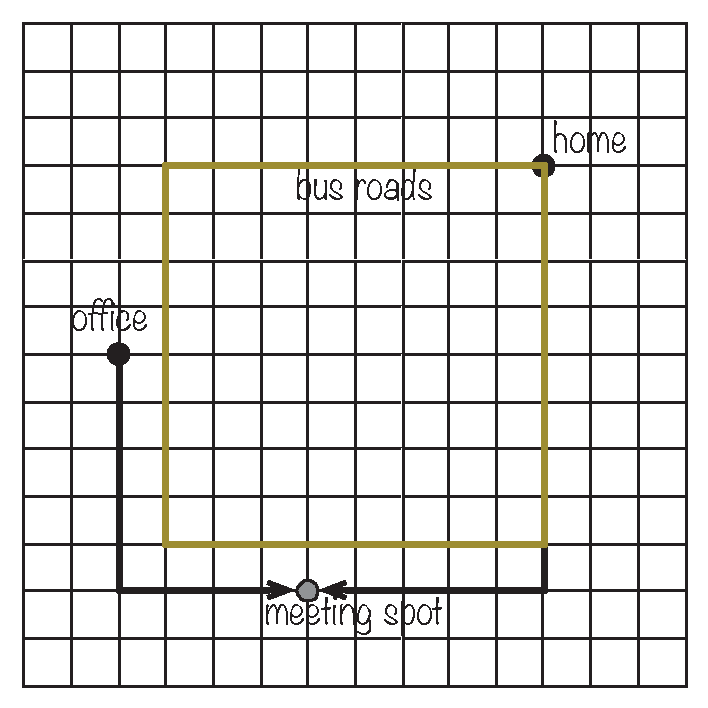
\includegraphics[width=2.7in]{paper-MPAR/Manhattan}
\caption{Working day movement模型,结合Manhattan blocks.}
\label{fig:chap3_manhattan}
\end{figure}

网络场景设定如下。行人数量分别设为200, 400, 600, 800。公交车,办公室及活动场所的数量分别设为总节点数目的2\%, 20\%, 2.5\%。在模拟器时间内,每人每天工作时间设为8小时。每人晚上参加夜晚活动的概率为0.5。此外,每个人有车的概率为0.2,若有车,则晚上参加活动将会开车,否则将乘巴士。行人的行走速度设为0.8--1.4m/s。如\figurename~\ref{fig:chap3_manhattan}所示,网络中设有三类地点,家(home),办公室(office)及聚会地点(meeting spot)。在街区中心设有一个环绕中心的公交路线,可以用于搭载行人。在每一个家,办公室及聚会地点,都设有一个throw-box,用以接管和传递消息。所有节点都以蓝牙接口通信,传输半径设为10 m,数据率设为250 KB/s。由于每一类地点(家,办公室或聚会地点)都设为地图上的一个点,仿真中确保每个节点到达这些地点后一定与throwbox发生接触。在仿真中,共产生30,000条消息,对于每条消息,其源节点和目的节点从所有行人节点中随机选择。每条消息的大小设为500 K 至 1 M 之间。仿真区域的大小根据节点数目的多少按同比例设定。对于整个仿真过程,其仿真器时间设为12天。

本节将MPAR算法与两个经典算法相比较:Delegation Forwarding (DF) \upcite{Erramilli2008}与Simbet \upcite{Daly2007}。采用四项评估指标:投递率(delivery ratio),平均时延(average latency),网络开销(overhead ratio)及平均每跳数(average hop count)。



\subsection{改变消息生存时间}

节点缓存大小固定在200M。消息的生存时间在10小时到30小时变化,仿真结果如\figurename~\ref{fig:chap3_delivery_ttl},\figurename~\ref{fig:chap3_latency_ttl},\figurename~\ref{fig:chap3_overhead_ttl},\figurename~\ref{fig:chap3_hop_ttl}。

仿真结果表明,两种MPAR算法,Local-MPAR及Tabu-MPAR,其性能表现都要优于DF及SimBet。与DF算法相比,Tabu-MPAR和Local-MPAR分别可以增加约71.1\%及37.8\%的消息投递率,且能降低约83.8\%及57.8\%的平均时延。与SimBet算法相比,Tabu-MPAR和Local-MPAR分别可以增加95.2\%和55.3\%的投递率,且能降低大概79.2\%及60.1\%的平均时延。从\figurename~\ref{fig:chap3_overhead_ttl}可以看出,Tabu-MPAR和Local-MPAR具有比DF及SimBet更低的网络开销。对于三中社会属性相关的路由算法,Tabu-MPAR, Local-MPAR及SimBet而言,网络开销要比DF低很多,特别是在消息生存时间设为比较长时。当网络中节点数目更小时,这种提升就越明显。由于MPAR路由算法限制了消息的最大副本数量,且利用throwbox辅助投递消息,中继传输操作非常少。此外,随着节点数目的增加,对于每个节点而言,其开销也会相应减小,导致整个网络的开销减小。\figurename~\ref{fig:chap3_hop_ttl}显示了消息平均跳数的性能表现。可以看出,两种MPAR算法具有比DF和SimBet更低的平均跳数。当节点数目增加时,平均跳数也增加;其原因是仿真区域按同比例增加后,需要节点间更多的合作,用以投递消息。



\subsection{改变节点缓存大小}

消息生存时间固定为仿真器中的16小时。节点缓存大小在50 MB 到 300 MB 之间变换。仿真结果如\figurename~\ref{fig:chap3_delivery_buffer},\figurename~\ref{fig:chap3_latency_buffer},\figurename~\ref{fig:chap3_overhead_buffer},\figurename~\ref{fig:chap3_hop_buffer}。

仿真结果表明,两种MPAR算法,Local-MPAR及Tabu-MPAR,其性能表现皆优于DF及SimBet。与DF算法相比,Tabu-MPAR和Local-MPAR分别可以增加约83.8\%及40.3\%的消息投递率,且能降低约83.8\%及57.8\%的平均时延。与SimBet算法相比,Tabu-MPAR和Local-MPAR分别可以增加3倍和2.5的投递率,且能降低大概80\%及60\%的平均时延。从\figurename~\ref{fig:chap3_overhead_buffer}可以看出,Tabu-MPAR和Local-MPAR具有几乎相同的网络开销;当缓存大小设为120 MB 时,MPAR算法的网络开销比SimBet略低一点,比DF低很多。当网络中节点数目更小时,性能提升越明显,如\figurename~\ref{fig:chap3_overhead_buffer}所示。与消息生存时间作为变量时相同,从\figurename~\ref{fig:chap3_hop_buffer}可以看出,两种MPAR算法具有比DF和SimBet更低的消息平均跳数,且当节点数目增加时,平均跳数也随之增加。


\begin{figure}[htbp]
\centering
\subfigure[Number of nodes: $|\overline{N}|=200$\label{200_delivery_ttl}]
{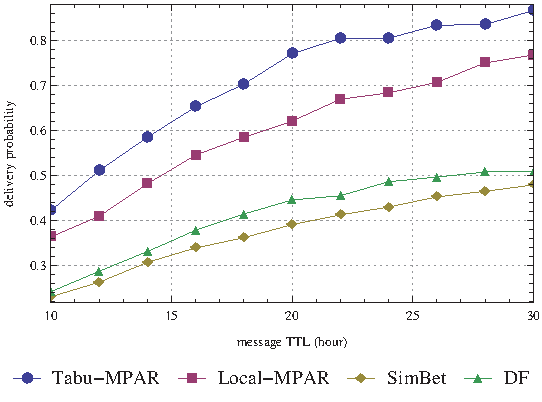
\includegraphics[width=0.37\textwidth]{paper-MPAR/200_delivery_ttl}}\quad\quad
\subfigure[Number of nodes: $|\overline{N}|=400$\label{400_delivery_ttl}]
{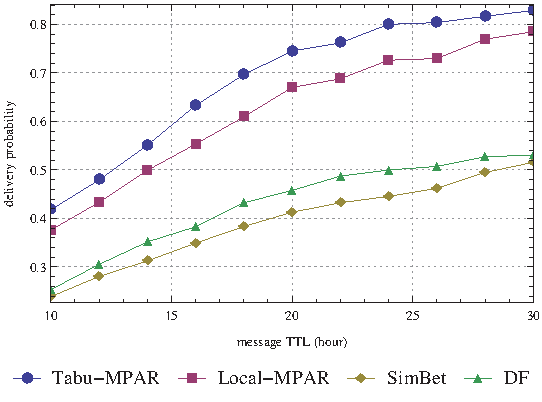
\includegraphics[width=0.37\textwidth]{paper-MPAR/400_delivery_ttl}} \\
\subfigure[Number of nodes: $|\overline{N}|=600$\label{600_delivery_ttl}]
{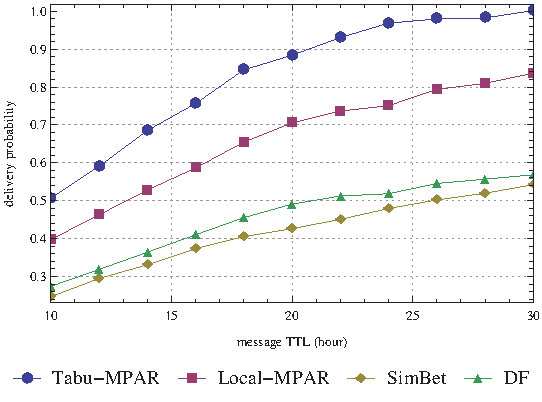
\includegraphics[width=0.37\textwidth]{paper-MPAR/600_delivery_ttl}}\quad\quad
\subfigure[Number of nodes: $|\overline{N}|=800$\label{800_delivery_ttl}]
{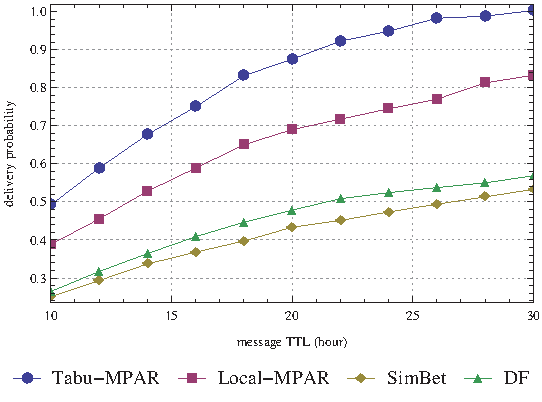
\includegraphics[width=0.37\textwidth]{paper-MPAR/800_delivery_ttl}}
\caption{消息投递率 vs. 消息生存时间}
\label{fig:chap3_delivery_ttl}
\end{figure}

\begin{figure}[htbp]
\centering
\subfigure[Number of nodes: $|\overline{N}|=200$\label{200_avgLatency_ttl}]
{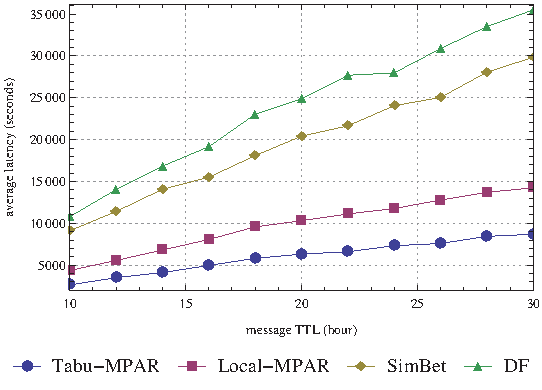
\includegraphics[width=0.37\textwidth]{paper-MPAR/200_avgLatency_ttl}}\quad\quad
\subfigure[Number of nodes: $|\overline{N}|=400$\label{400_avgLatency_ttl}]
{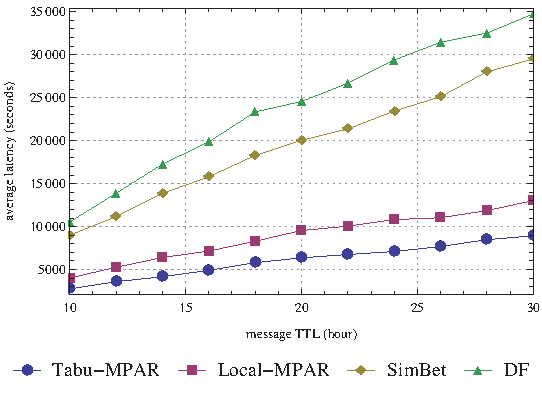
\includegraphics[width=0.37\textwidth]{paper-MPAR/400_avgLatency_ttl}} \\
\subfigure[Number of nodes: $|\overline{N}|=600$\label{600_avgLatency_ttl}]
{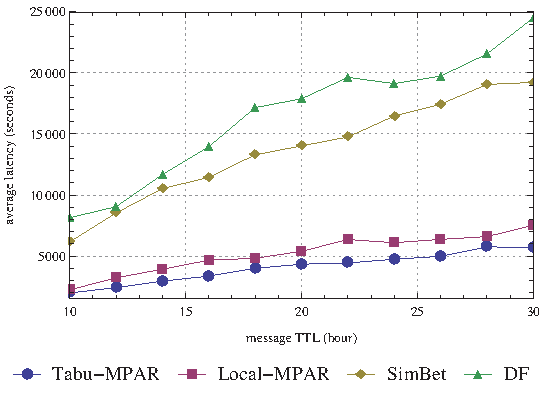
\includegraphics[width=0.37\textwidth]{paper-MPAR/600_avgLatency_ttl}}\quad\quad
\subfigure[Number of nodes: $|\overline{N}|=800$\label{800_avgLatency_ttl}]
{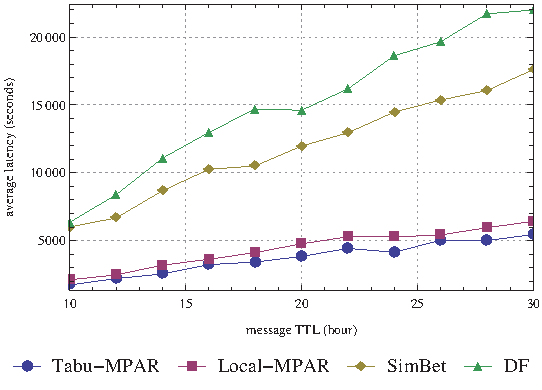
\includegraphics[width=0.37\textwidth]{paper-MPAR/800_avgLatency_ttl}}
\caption{端到端平均时延 latency vs. 消息生存时间}
\label{fig:chap3_latency_ttl}
\end{figure}

\begin{figure}[htbp]
\centering
\subfigure[Number of nodes: $|\overline{N}|=200$\label{200_overhead_ttl}]
{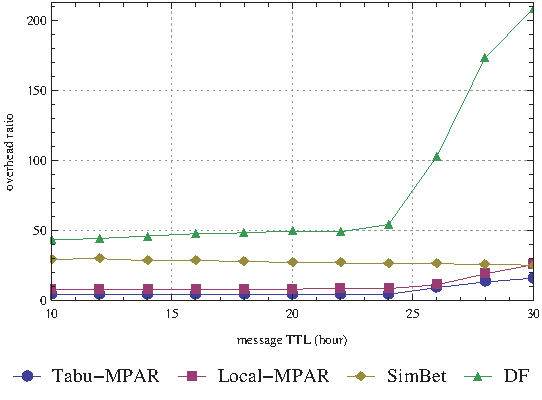
\includegraphics[width=0.37\textwidth]{paper-MPAR/200_overhead_ttl}}\quad\quad
\subfigure[Number of nodes: $|\overline{N}|=400$\label{400_overhead_ttl}]
{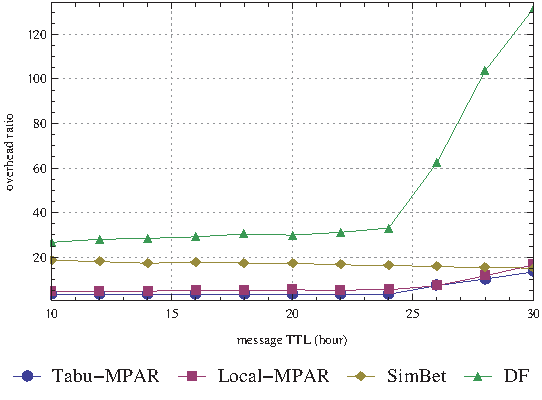
\includegraphics[width=0.37\textwidth]{paper-MPAR/400_overhead_ttl}} \\
\subfigure[Number of nodes: $|\overline{N}|=600$\label{600_overhead_ttl}]
{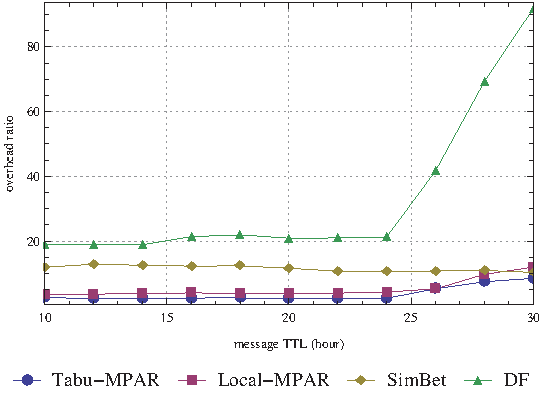
\includegraphics[width=0.37\textwidth]{paper-MPAR/600_overhead_ttl}}\quad\quad
\subfigure[Number of nodes: $|\overline{N}|=800$\label{800_overhead_ttl}]
{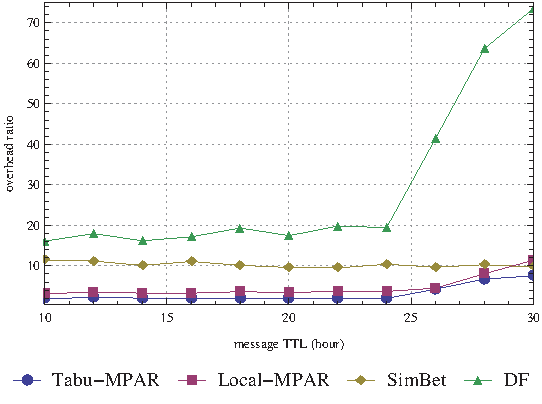
\includegraphics[width=0.37\textwidth]{paper-MPAR/800_overhead_ttl}}
\caption{网络开销 vs. 消息生存时间}
\label{fig:chap3_overhead_ttl}
\end{figure}

\begin{figure}[htbp]
\centering
\subfigure[Number of nodes: $|\overline{N}|=200$\label{200_avgHop_ttl}]
{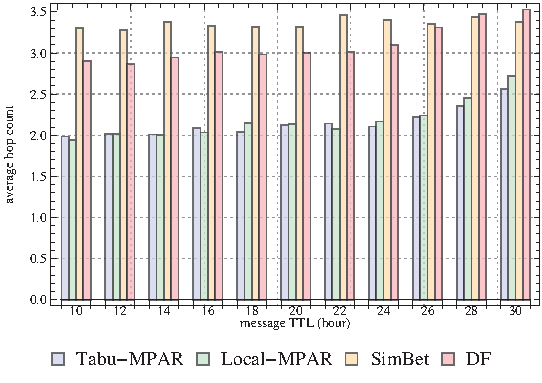
\includegraphics[width=0.37\textwidth]{paper-MPAR/200_avgHop_ttl}}\quad\quad
\subfigure[Number of nodes: $|\overline{N}|=400$\label{400_avgHop_ttl}]
{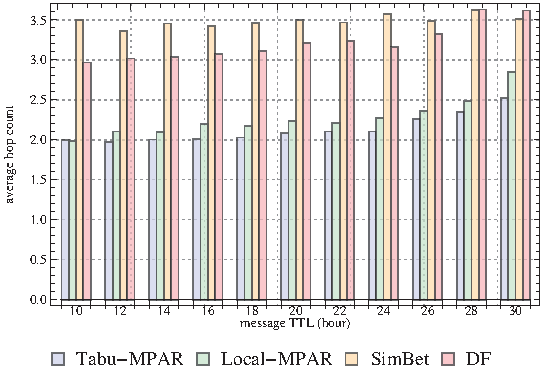
\includegraphics[width=0.37\textwidth]{paper-MPAR/400_avgHop_ttl}} \\
\subfigure[Number of nodes: $|\overline{N}|=600$\label{600_avgHop_ttl}]
{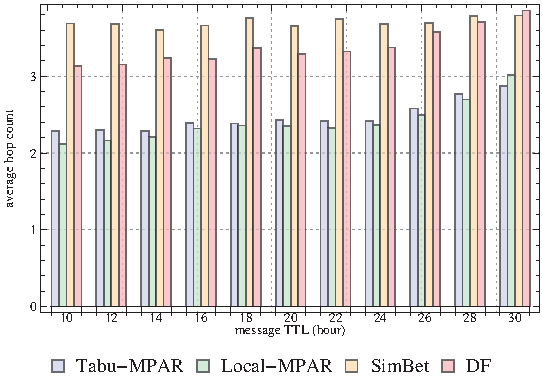
\includegraphics[width=0.37\textwidth]{paper-MPAR/600_avgHop_ttl}}\quad\quad
\subfigure[Number of nodes: $|\overline{N}|=800$\label{800_avgHop_ttl}]
{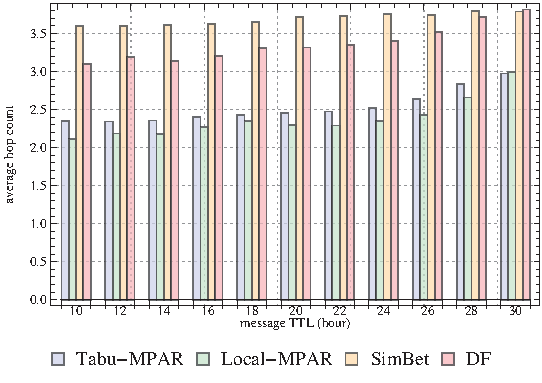
\includegraphics[width=0.37\textwidth]{paper-MPAR/800_avgHop_ttl}}
\caption{平均跳数 vs. 消息生存时间}
\label{fig:chap3_hop_ttl}
\end{figure}

\begin{figure}[htbp]
\centering
\subfigure[Number of nodes: $|\overline{N}|=200$\label{200_delivery_buffer}]
{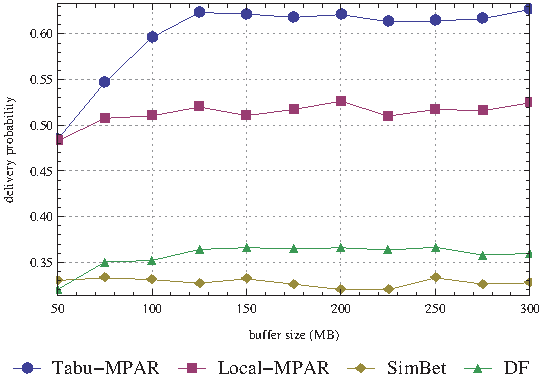
\includegraphics[width=0.37\textwidth]{paper-MPAR/200_delivery_buffer}}\quad\quad
\subfigure[Number of nodes: $|\overline{N}|=400$\label{400_delivery_buffer}]
{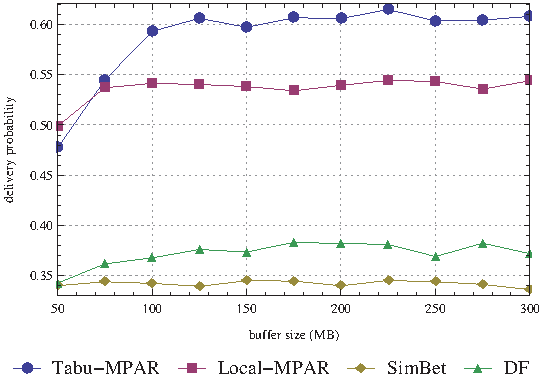
\includegraphics[width=0.37\textwidth]{paper-MPAR/400_delivery_buffer}} \\
\subfigure[Number of nodes: $|\overline{N}|=600$\label{600_delivery_buffer}]
{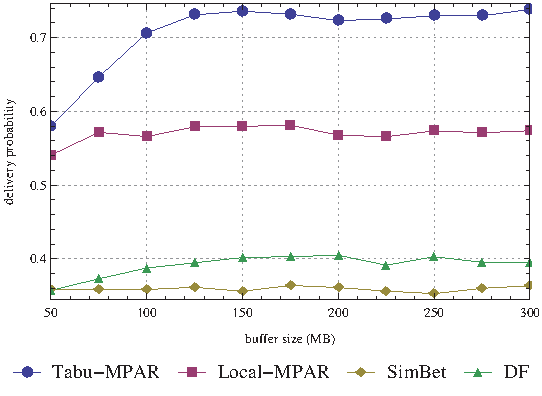
\includegraphics[width=0.37\textwidth]{paper-MPAR/600_delivery_buffer}}\quad\quad
\subfigure[Number of nodes: $|\overline{N}|=800$\label{800_delivery_buffer}]
{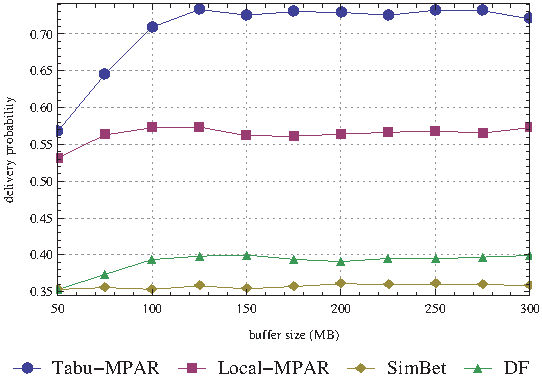
\includegraphics[width=0.37\textwidth]{paper-MPAR/800_delivery_buffer}}
\caption{消息投递率 vs. 节点缓存}
\label{fig:chap3_delivery_buffer}
\end{figure}

\begin{figure}[htbp]
\centering
\subfigure[Number of nodes: $|\overline{N}|=200$\label{200_avgLatency_buffer}]
{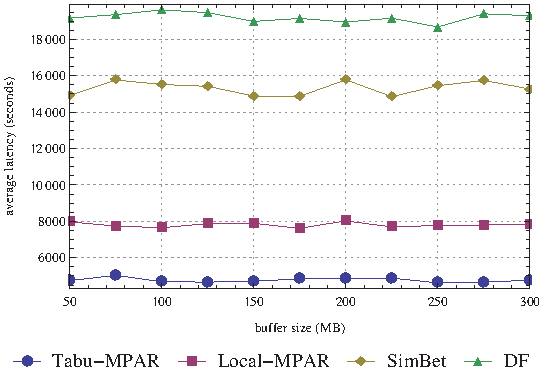
\includegraphics[width=0.37\textwidth]{paper-MPAR/200_avgLatency_buffer}}\quad\quad
\subfigure[Number of nodes: $|\overline{N}|=400$\label{400_avgLatency_buffer}]
{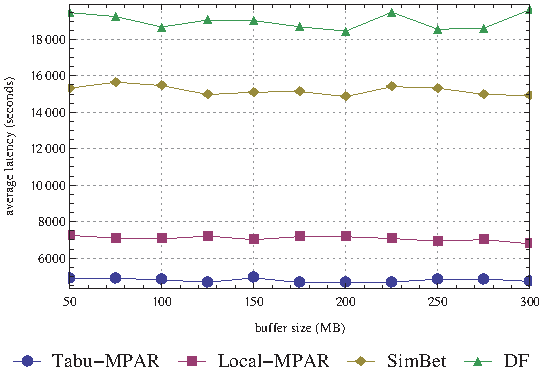
\includegraphics[width=0.37\textwidth]{paper-MPAR/400_avgLatency_buffer}} \\
\subfigure[Number of nodes: $|\overline{N}|=600$\label{600_avgLatency_buffer}]
{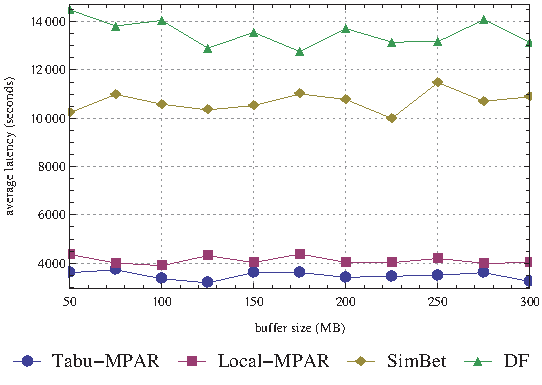
\includegraphics[width=0.37\textwidth]{paper-MPAR/600_avgLatency_buffer}}\quad\quad
\subfigure[Number of nodes: $|\overline{N}|=800$\label{800_avgLatency_buffer}]
{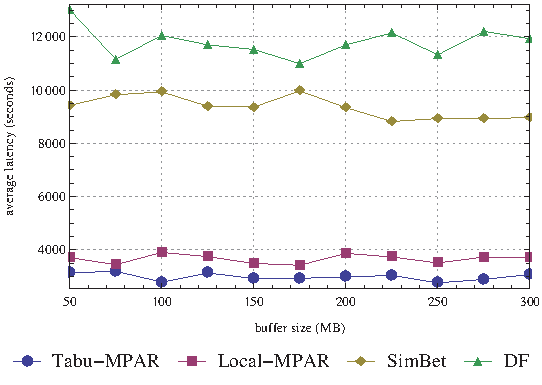
\includegraphics[width=0.37\textwidth]{paper-MPAR/800_avgLatency_buffer}}
\caption{端到端平均时延 vs. 节点缓存}
\label{fig:chap3_latency_buffer}
\end{figure}

\begin{figure}[htbp]
\centering
\subfigure[Number of nodes: $|\overline{N}|=200$\label{200_overhead_buffer}]
{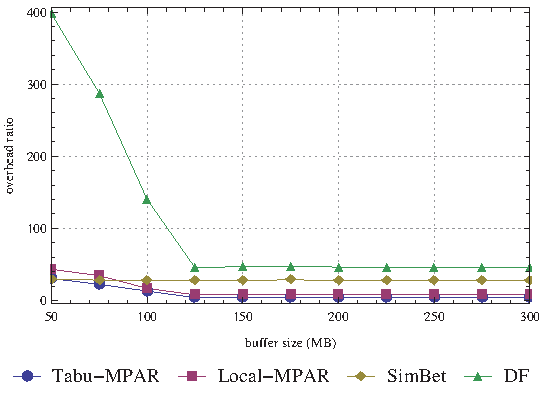
\includegraphics[width=0.37\textwidth]{paper-MPAR/200_overhead_buffer}}\quad\quad
\subfigure[Number of nodes: $|\overline{N}|=400$\label{400_overhead_buffer}]
{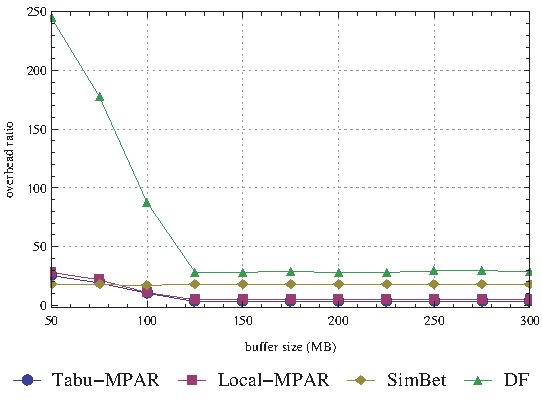
\includegraphics[width=0.37\textwidth]{paper-MPAR/400_overhead_buffer}} \\
\subfigure[Number of nodes: $|\overline{N}|=600$\label{600_overhead_buffer}]
{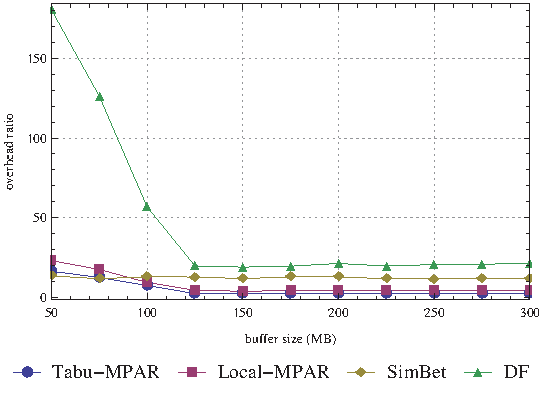
\includegraphics[width=0.37\textwidth]{paper-MPAR/600_overhead_buffer}}\quad\quad
\subfigure[Number of nodes: $|\overline{N}|=800$\label{800_overhead_buffer}]
{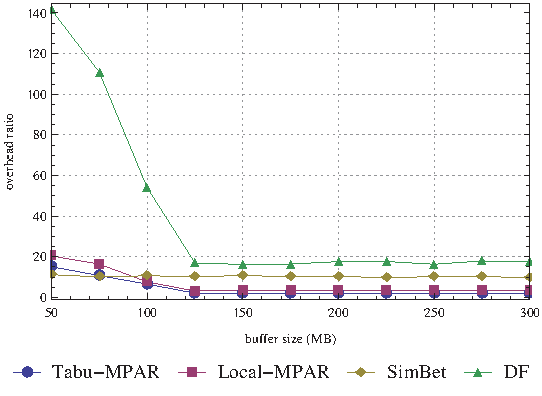
\includegraphics[width=0.37\textwidth]{paper-MPAR/800_overhead_buffer}}
\caption{网络开销 vs. 节点缓存}
\label{fig:chap3_overhead_buffer}
\end{figure}

\begin{figure}[htbp]
\centering
\subfigure[Number of nodes: $|\overline{N}|=200$\label{200_avgHop_buffer}]
{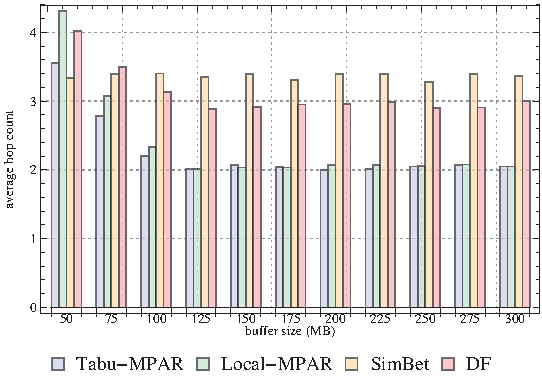
\includegraphics[width=0.37\textwidth]{paper-MPAR/200_avgHop_buffer}}\quad\quad
\subfigure[Number of nodes: $|\overline{N}|=400$\label{400_avgHop_buffer}]
{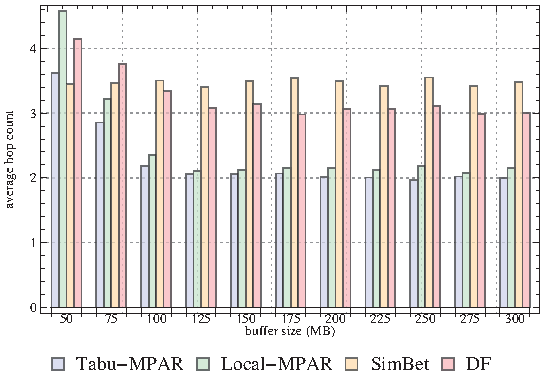
\includegraphics[width=0.37\textwidth]{paper-MPAR/400_avgHop_buffer}} \\
\subfigure[Number of nodes: $|\overline{N}|=600$\label{600_avgHop_buffer}]
{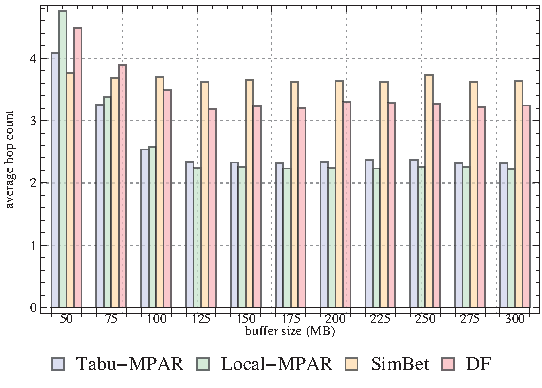
\includegraphics[width=0.37\textwidth]{paper-MPAR/600_avgHop_buffer}}\quad\quad
\subfigure[Number of nodes: $|\overline{N}|=800$\label{800_avgHop_buffer}]
{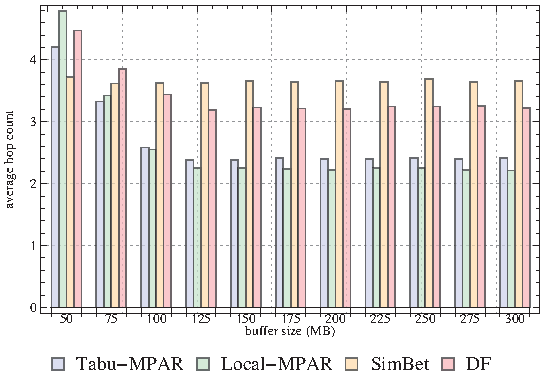
\includegraphics[width=0.37\textwidth]{paper-MPAR/800_avgHop_buffer}}
\caption{平均跳数 vs. 节点缓存}
\label{fig:chap3_hop_buffer}
\end{figure}



\section{本章小结}
\label{chap3:本章总结}
在本章中,建立了周期相关的移动记录模型,并从移动记录中提取出节点(群组)移动模式。对于成组的节点,其被看做一个整体,并评估整体的预测投递率。本章研究了两个相关路由的关键属性,并将路由问题建模为组合最优化问题,且证明了该问题的$\mathcal{NP}$难解性。为求解该路由问题,基于局部搜索及禁忌搜索,分别提出了两种路由算法Local-MPAR及Tabu-MPAR。此外,本章证明了Tabu-MPAR过程可以使得持有消息的节点集合最终达到预测投递概率最优的集合。仿真实验表明,两种MPAR算法,在机会网络中的综合移动模型WDM上优于DF算法及SimBet算法。

~\\
~\\
~\\
~\\
~\\
~\\
~\\
~\\
~\\
~\\


